\documentclass[english, LaM, oneside]{sapthesis}%remove "english" for a thesis written in Italian
%Bachelor's (laurea triennale) thesis : Lau 
%Master's (laurea specialistica) thesis: LaM 
%PhD's thesis: PhD 
%\usepackage[italian]{babel} %use this package for a thesis written in Italian
\usepackage[utf8]{inputenx}
\usepackage{indentfirst}
\usepackage{microtype}
%\usepackage{chemformula}
%\usepackage{setspace}
%\usepackage{yfonts,color}
%\usepackage{siunitx}
%\usepackage{comment}
%\usepackage{multirow}
%\usepackage{varioref}
%\usepackage[bottom]{footmisc}
%\usepackage{wrapfig}
%\usepackage{float}
%\usepackage{type1cm}
\usepackage{csquotes}
\usepackage{lettrine}
\usepackage{cite}
\usepackage{amssymb}
\usepackage{amsmath}
\numberwithin{equation}{chapter}
\usepackage{booktabs}
\usepackage{graphicx}
\linespread{0.9}
%\usepackage{chngcntr}
\usepackage[nottoc, notlof, notlot]{tocbibind}
%\onehalfspacing
%\counterwithout{footnote}{chapter}
\usepackage{hyperref}
\usepackage{tabularx}
\hypersetup{
			hyperfootnotes=true,			
			bookmarks=true,			
			colorlinks=true,
			linkcolor=red,
                        linktoc=page,
			anchorcolor=black,
			citecolor=red,
			urlcolor=blue,
			pdftitle={Evaluating Pre-Trained Vision Transformers Under Continual Learning},
			pdfauthor={Swati Aggrawal},
			pdfkeywords={thesis, sapienza, roma, university}
 }

\title{Evaluating Pre-Trained Vision Transformers Under Continual Learning}
\author{Swati Aggrawal}
\IDnumber{2118031}
\course[]{Computer Science}
\courseorganizer{Facoltà di Ingegneria dell’Informazione, Informatica e Statistica}
\submitdate{2025/2026}
\copyyear{2026}
\advisor{Prof. Maria De Marsico}
\coadvisor{Prof. Marco Raoul Marini}
\authoremail{swatiagg357@gmail.com}
% \examdate{22 September 2015}
% \examiner{Prof. ...} \examiner{Prof. ...} \examiner{Prof. ...}  \examiner{Prof. ...}  \examiner{Prof. ...} \examiner{Prof. ...}  \examiner{Prof. ...} 

%we refer to http://ctan.mirrorcatalogs.com/macros/latex/contrib/sapthesis/sapthesis-doc.pdf for an exhaustive description of the sapthesis documentclass.



\begin{document}

\frontmatter
\maketitle

% \clearpage
% \thispagestyle{empty}

% \vspace*{\fill}
% \begin{flushright}
% \itshape
% “Dedicated to my Family.”\\[1em]
% % --- Author Name
% \end{flushright}
% \vspace*{\fill}

% \clearpage

\begin{abstract}
Evaluating pre-trained Vision Transformers (ViTs) under Continual Learning (CL) is a largely underexplored area, as the majority of research in this field has historically focused on convolutional neural network architectures. This thesis examines that gap by systematically investigating how pre-trained ViT-Tiny behaves under sequential task learning, and whether targeted architectural and regularization modifications can reduce catastrophic forgetting, the tendency of neural networks to lose performance on previously learned tasks when trained on new ones.

The evaluation is conducted under a task-incremental CL framework on the Split CIFAR-100 benchmark, comprising five sequential tasks of twenty classes each. Four model configurations are assessed in a structured ablation chain: ImageNet pre-trained ResNet-18 and ViT-Tiny as naive sequential fine-tuning baselines, ViT-Tiny with bottleneck adapter modules as a parameter-efficient adaptation strategy, and the same adapter-based model augmented with Elastic Weight Consolidation (EWC) regularization applied exclusively to the adapter parameters.

The evaluation reveals a clear and progressive improvement across configurations. The method of freezing the pre-trained ViT model and directing learning through lightweight adapters achieves a drastic reduction in forgetting by restricting gradient update computations to only 5.5\% of all parameters. The addition of EWC further stabilises knowledge retention across the task sequence, achieving strong average accuracy with minimal forgetting. Evaluation across three random seeds suggests that these results are consistent across different task orderings and class partitions.

Together, the findings suggest that pre-trained ViTs, when evaluated under a CL framework with appropriate parameter-efficient and regularization strategies, can achieve strong sequential task performance with minimal catastrophic forgetting.
\end{abstract}

\tableofcontents

\mainmatter
\chapter{Introduction}
 This chapter is intended to provide background and context for this study. The motivation for this research and the fundamental question it seeks to answer are outlined in section \ref{sec:1.1}. The existing body of work on ViTs and CL is discussed in section \ref{sec:1.2}, with particular emphasis on important breakthroughs and limitations. Finally, section \ref{sec:1.3} concludes by summarizing the major contributions of this thesis while also summarizing the content of the rest of this work.
\section{Aim and Scope}
\label{sec:1.1}
For a human being, learning is a continuous process in which new information is obtained without discarding the previously acquired knowledge. For Artificial Neural Networks (ANNs), this kind of ability is challenging due to the problem of catastrophic forgetting, a phenomenon that significantly affects performance when models are trained multiple times on different tasks\cite{1}\cite{2}. To counter this problem, CL developed methods that helped models retain previously acquired knowledge while adapting to new information. As artificial intelligence (AI) systems are used more and more in the real world, the capacity to learn gradually is becoming more and more crucial.

Convolutional Neural Networks (CNNs), such as ResNet, have always been the preferred solution for image classification tasks in the domain of Computer Vision (CV)\cite{3}. However, the focus is currently on the development of transformer-based models for image classification tasks by leveraging the benefits of self-attention techniques, as introduced in ViT architectures\cite{4}. Although ViTs have demonstrated competitive or better performance in extensive supervised learning tests, relatively little is known about how persistent and flexible they are in CL environments\cite{5}.

The aim of this thesis work is to apply a task-incremental CL framework to comprehensively assess the performance of pre-trained ViTs. This study investigates their performance on a number of sequential learning tasks and compares it to pre-defined convolutional baselines. In addition, the transformer architecture has been incorporated with lightweight adapter modules to ensure maximum flexibility and minimize parameter updates. To overcome the problem of catastrophic forgetting, EWC is also applied as a regularization method. With these enhancements, the study investigates how architectural modifications and methods of CL impact performance and memory retention.

It is important to clarify that this thesis evaluates pre-trained ViTs as they are most commonly deployed in practice as frozen feature extractors adapted via lightweight modules. The research question is not whether ViTs can learn sequentially from random initialization, but whether pre-trained ViTs, combined with parameter-efficient adaptation strategies, can serve as effective CL systems. The naive fine-tuning baseline (as shown in Section \ref{sec:5.1}) establishes the sequential learning behavior of ViT-Tiny without any freezing, providing a reference point against which the frozen adapter approach is compared.

The scope of this work is related to supervised image classification in a controlled CL environment. The performance of the model is compared through various quantitative measures such as average accuracy, average forgetting, and Backward Transfer (BWT). To understand the applicability of the already pre-trained transformer-based architectures in sequential learning and whether certain modifications can be made to improve the stability of these architectures over time, this thesis attempts to compare the baseline and improved model in a systematic manner.
\section{State of the Art}
\label{sec:1.2}
The objective of CL, an important area of Machine Learning (ML) research\cite{6}, is the capacity of the model to learn in succession from the flow of tasks without forgetting previously learned information.  CL represents more realistic scenarios in which the model has access to data over time, as opposed to the traditional training paradigm, in which the model is trained on the data once. Catastrophic forgetting, in which Neural Networks perform substantially worse on the previously learned tasks after learning new tasks, represents an important challenge in this context. The use of intelligent systems in realistic scenarios, in which adaptability and the retention of information are crucial, it is therefore vital to tackle this problem.

Several kinds of strategies have been put into practice over time for minimizing catastrophic forgetting in CL. The majority of these techniques fall under the following primary categories:
\begin{itemize}
    \item Regularization based methods: Using penalty terms, restrict parameter updates to preserve prior knowledge. EWC\cite{2} and MAS\cite{7} assess the relevance of parameters, but distillation-based methods maintain output behavior across tasks\cite{8}.
    \item Replay based methods: Forgetting can be reduced by reviewing previously collected information. Experience replay saves exemplars (e.g., iCaRL\cite{9}), whereas generative replay approximates former task distributions by synthesizing samples using models such as MeRGAN\cite{10}.
    \item Architectural methods: Modify the model's structure by incorporating routing approaches or expanding capacity. Transformers can be incrementally extended using techniques like DyTox\cite{11}, which increase scalability but often raises model complexity.
    \item Hybrid methods: For better stability–plasticity trade-off, combining prompting, replay, distillation, or architectural growth can led to better results. CL-DETR\cite{12} and iCaRL\cite{9} are two examples of integrated approaches for challenging vision-based CL tasks.
\end{itemize}

\begin{figure}[!htbp]
    \centering
    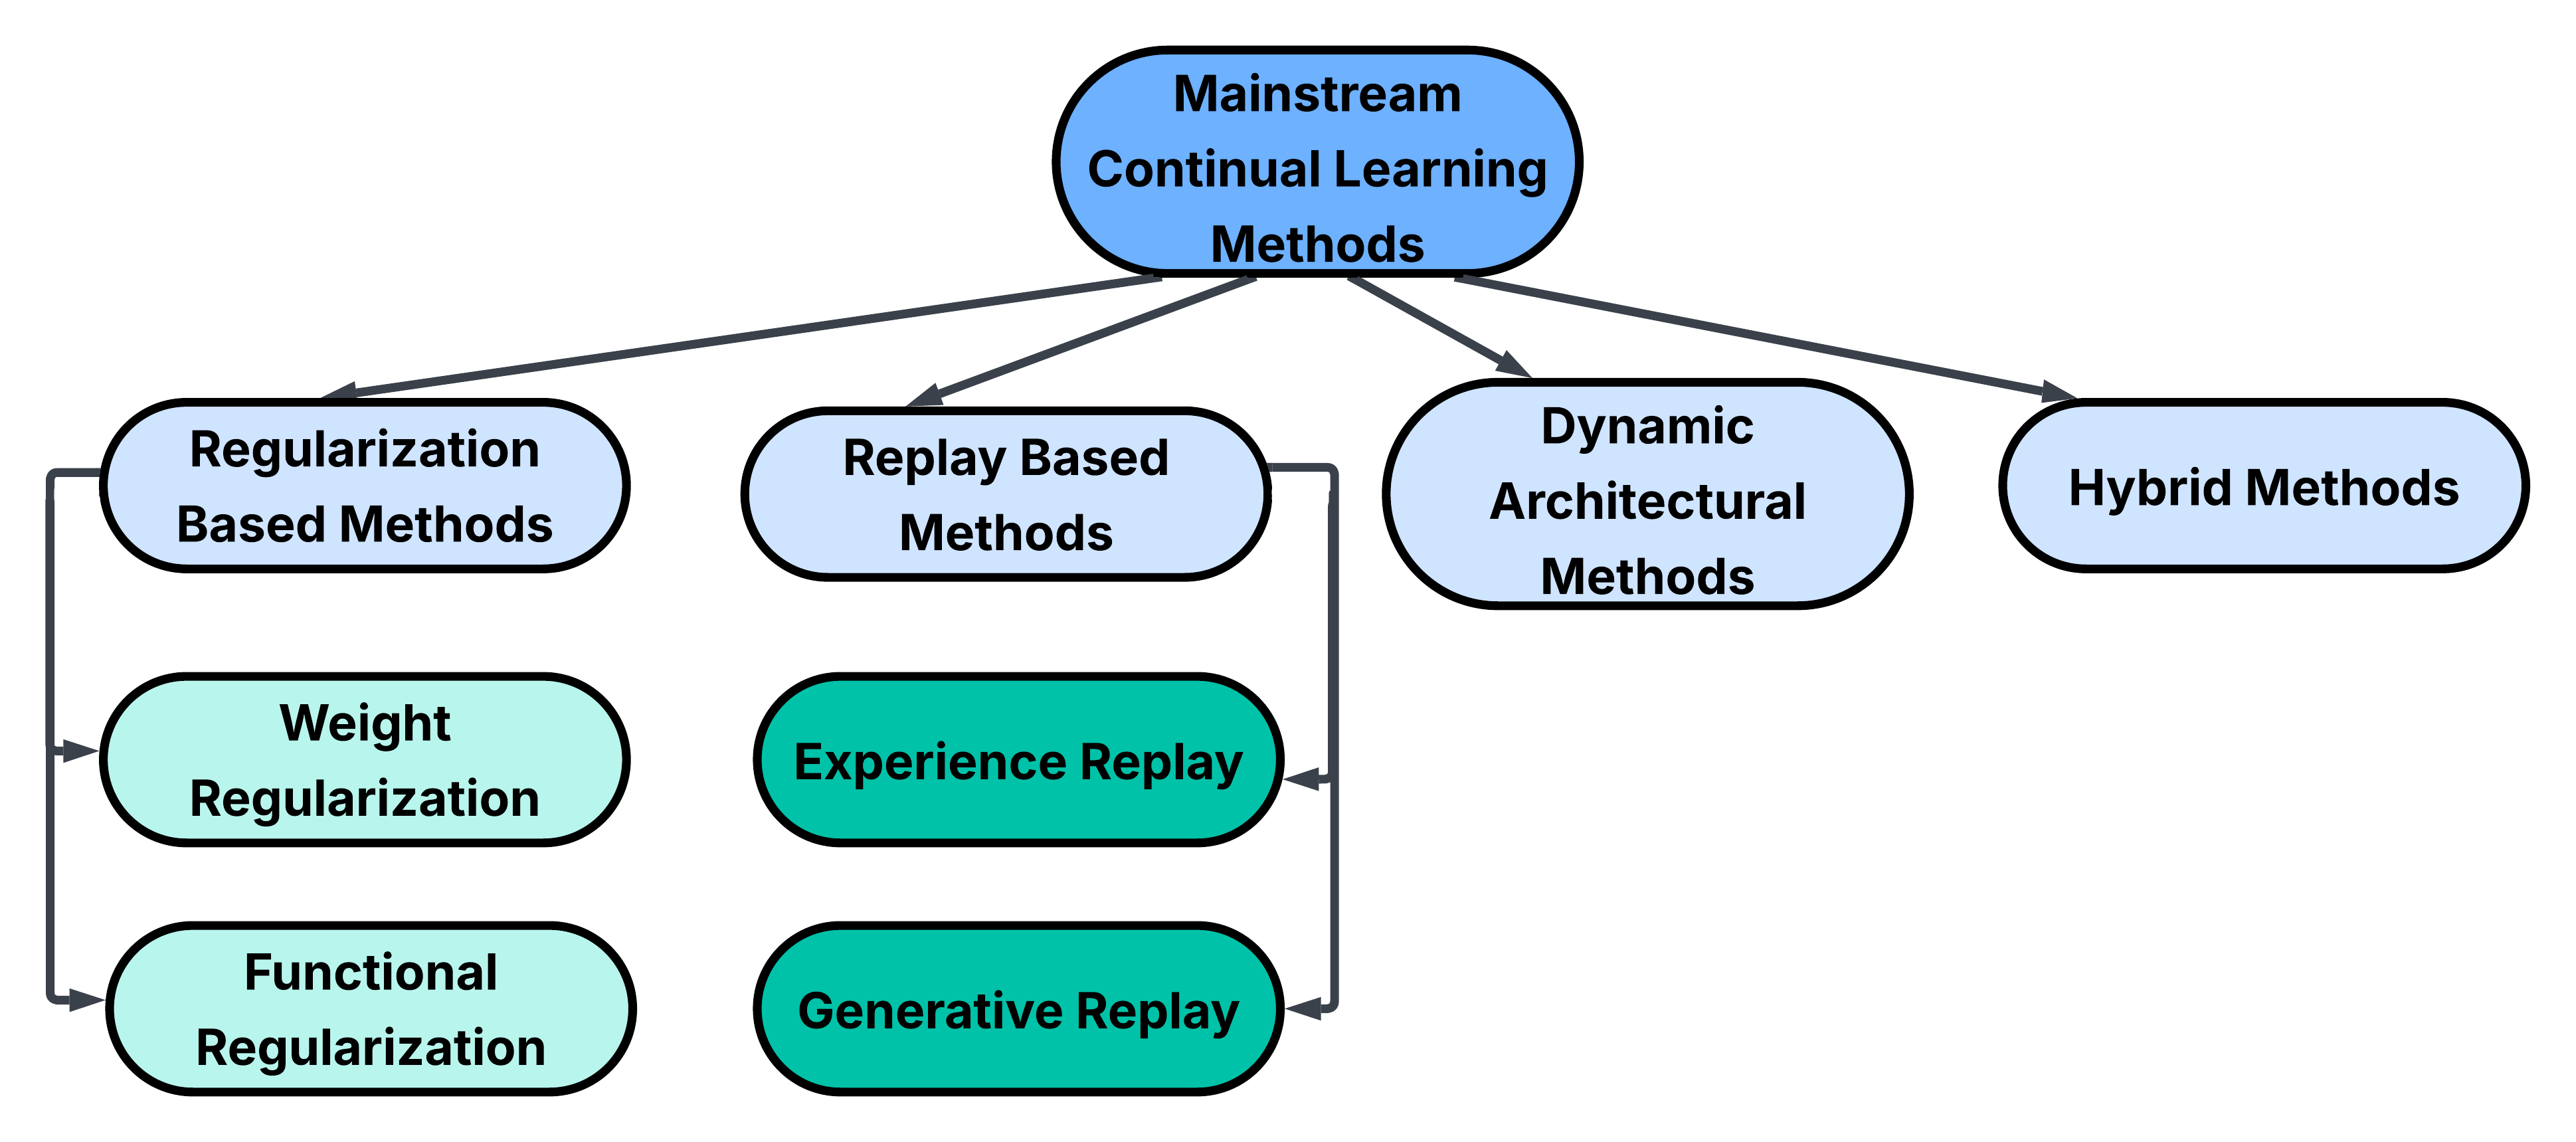
\includegraphics[width=\textwidth]{clstrategies.png}
    \caption{ Taxonomy of mainstream CL methods categorized into
regularization-based, replay-based, dynamic architectural, and hybrid approaches.}
    \label{fig:clstrategies}
\end{figure}


More recently, prompt-based methods have emerged as a dominant paradigm for applying pre-trained ViTs to CL. The Learning to Prompt (L2P) method \cite{5} proposed a prompt pool that conditioned the frozen ViT using task-relevant prompts drawn from a key-value memory learned during training, thereby attaining impressive CL results without fine-tuning the model parameters. The DualPrompt framework \cite{41} further improved on this idea by breaking down prompts into two categories, G-Prompt and E-Prompt, which are task agnostic and task specific, respectively. These methods are architecturally distinct from adapter-based approaches: prompts operate at the input token level, while adapters modify intermediate representations. Taking a different approach, SLCA (Slow Learner with Classifier Alignment)\cite{slca} has demonstrated that careful management of the learning rate schedule and classifier alignment on frozen pre-trained ViTs yields strong CL baselines, addressing classifier bias that arises from imbalanced task exposure. A related line of work explores tuning only the normalization layers for CL. Pham et al.\cite{pham} proposed Continual Normalization as a replacement for Batch Normalization in online CL, showing that standard BN statistics become biased towards the current task during sequential training and contribute to forgetting. Motivated by similar insights, De Min et al.\cite{demin} demonstrated that tuning solely the LayerNorm scale and bias parameters of a frozen ViT achieves results competitive with prompt-based methods while being significantly more parameter-efficient, representing a complementary alternative to adapter-based approaches.

It is important to note that these methods operate under substantially different experimental conditions from those adopted in this thesis, making direct numerical comparison misleading. L2P \cite{5}, DualPrompt\cite{41} and SLCA\cite{slca} use a ViT-B/16 backbone with 86 million parameters pre-trained on ImageNet-21K, a dataset of approximately 14 million images across 21,841 classes. They evaluate under the Class Incremental Learning (CIL) scenario with ten tasks of ten classes each on Split CIFAR-100, where task identity is unavailable at test time and the model must discriminate among all seen classes jointly. In contrast, this thesis uses a ViT-Tiny backbone with 5.85 million parameters pre-trained on ImageNet-1K, evaluates under the less demanding TIL scenario with five tasks of twenty classes each, and provides task identity at inference time. The adaptation strategies also differ fundamentally: L2P \cite{5} and DualPrompt\cite{41} operate at the input token level by prepending learnable prompts, while the adapter-based approach in this thesis modifies intermediate representations within each Transformer block. These differences in backbone capacity, pre-training data, CL scenario, and adaptation mechanism mean that the contribution of this thesis should be understood as a systematic investigation of adapter-based PEFT combined with EWC regularisation in the TIL setting, rather than as a direct competitor to these CIL-focused methods.

Having situated the prompt-based and adapter-based approaches within the current state-of-the-art landscape, the following is a preview of the architectural foundations, CNNs and ViTs that underpin these methods and explain why ViTs in particular are well-suited to CL research.

For many years, the development of CV has relied extensively on CNNs\cite{13}. Deep architectures were demonstrated by models such as ResNet\cite{3} to be able to train on images and perform well on a variety of classification and recognition tasks. They are robust and commonly used because of their design, which enables them to successfully capture regional patterns.

CNNs have drawbacks, nevertheless, in environments that require continuous learning. Sequential training tends to drive them to forgetting , which lowers performance on prior tasks. Although they perform well in typical training setups still this leaves them at risk of catastrophic forgetting\cite{14}.
These days, ViTs are a powerful alternative for CNNs\cite{4}. As mentioned before self-attention mechanisms allow models to record relationships across the full input and prioritize the most essential elements of an image. Additionally, this ability could mitigate forgetting when learning new data\cite{5}. Pretraining on large datasets makes them especially effective at recognition tasks. ViTs in this context are still mainly understudied because the majority of CL research to date has concentrated on CNNs. They are an intriguing choice for research on sequential learning scenarios because of their unique information processing approach.

When working with a transformer model, as the model grows it becomes expensive to update all parameters for every new task and the model might become unstable\cite{15}. An easy substitute is provided by adapter modules. Small trainable layers are added to the network but the original weights are mostly left unaltered as opposed to fine-tuning the entire model\cite{15}. This helps maintain previously learnt representations and significantly lowers the number of updated parameters. When new tasks are introduced consecutively, adapters can offer more stable learning because the majority of the pre-trained backbone remains in place. Because of this, they are particularly appealing for CL, where it is crucial to regulate how much the model changes.

The majority of CL techniques were designed and evaluated using CNN-based models, despite the fact that many other methods have been proposed\cite{6}. Meanwhile, ViT has demonstrated impressive results in common CV tasks, particularly when pre-trained on sizable datasets. The systematic assessment of pre-trained ViTs in Task-incremental Learning (TIL) environments is currently insufficient\cite{5}. For instance, the extent to which these models retain previous knowledge after sequential training is still underexplored.

Also, techniques like EWC are extensively researched for lowering forgetting, nothing is known about how they interact with parameter-efficient strategies like adapters. Whether using adapters alongside EWC increases stability, decreases forgetting, or creates new trade-offs has not been well studied. Therefore, to have a better understanding of how these elements interact, a systematic comparison is required.

By systematically examining pre-trained ViTs in a CL environment, this thesis fills in these gaps. Furthermore, it investigates the effects of EWC and adapter modules on forgetting, performance, and stability across sequential tasks.

\section{Contribution and thesis outline}
\label{sec:1.3}
In this work the problem of catastrophic forgetting is examined in pre-trained ViTs under CL. The choice of adapter modules over prompt-based methods such as L2P\cite{5} or DualPrompt\cite{41} is motivated by the goal of studying the interaction between parameter-efficient adaptation and explicit weight regularization via EWC. Adapters provide a well-defined, localized parameter space on which Fisher-based importance estimation can be applied directly, making the EWC + Adapter combination analytically cleaner than EWC applied to input-level prompts. Nevertheless, prompt-based methods represent an important line of work in CL and should be acknowledged as a relevant alternative design paradigm. 

Understanding how regularization techniques and parameter-efficient modifications affect performance and forgetting when tasks are learned sequentially is the primary objective of this study. More particularly, a systematic and comparative analysis of the relationship between adapter modules and EWC is performed.
The contributions of this thesis can be highlighted as follows:
\begin{itemize}
    \item A systematic evaluation of pre-trained ViT-Tiny under a task-incremental CL framework, providing insight into its forgetting behaviour and stability across sequential tasks compared to a CNN baseline.
    \item An investigation into parameter-efficient adaptation using bottleneck adapter modules, examining how freezing the backbone and limiting parameter updates affects performance and knowledge retention.
    \item An empirical analysis of combining adapter modules with EWC regularization, assessing whether applying EWC exclusively to adapter parameters improves the stability-plasticity balance over adapters alone.
    \item A structured ablation study across four model configurations, isolating the contribution of each component and demonstrating a clear and measurable progression in CL performance.
\end{itemize}

The rest of this thesis is organized as follows. \hyperref[chap:2]{Chapter~\ref*{chap:2}} introduces the basic concepts related to CL, such as how the problem is defined, how the performance is measured, and the basic strategies that are employed to address the problem. \hyperref[chap:3]{Chapter~\ref*{chap:3}} presents the Deep Learning (DL) architectures employed in this thesis, which include CNNs, ViTs, adapter modules, and EWC. \hyperref[chap:4]{Chapter~\ref*{chap:4}} presents the experimental setup, which includes the dataset, the configurations of the models, the training procedures, and the evaluation protocol. \hyperref[chap:5]{Chapter~\ref*{chap:5}} presents the results obtained by the four model configurations, along with an ablation study of the contribution of EWC and the results of the cross-validation analysis. \hyperref[chap:6]{Chapter~\ref*{chap:6}} concludes the thesis by highlighting the major findings and some suggestions for future work.
\chapter{CL: Concepts and Methods}
\label{chap:2}
Enabling models to learn from a series of tasks while maintaining knowledge from earlier tasks is the main goal of CL. In contrast when compared to conventional training, which functions under the assumption that data is static and independently distributed, CL works in dynamic environments where new data gradually becomes available. This presents problems like the stability-plasticity trade-off and catastrophic forgetting. The core ideas, evaluation metrics, and most common strategies that serve as the basis of current study on CL are presented in this chapter.
\section{CL Problem Definition}
The problem of training a model that is able to learn from a stream of data that is provided successively over time, as opposed to a fixed dataset, is a problem that CL seeks to solve\cite{6}. The presence of task boundaries, limited access to previously seen data, and the ability to update previously learned information in light of newly provided data requires a revision of the traditional supervised learning model in this domain. This section will provide a formal definition of the CL problem, including its optimization objective, typical experimental configurations, and the basic stability-plasticity trade-off of sequential learning systems.
\subsection{Learning Setup}
The regular supervised learning process is to use a dataset D to train the model.

\begin{equation}
    D=\left\{\left(x_i,y_i\right)\right\}_{i=1}^N
\end{equation}


where $x_i\in\mathrm{X}$ is the input space (images) and $y_i\in Y$ is the corresponding label. The process aims to achieve minimal empirical risk to obtain a parametric model $f_\theta:X\rightarrow Y$, with the parameters $\theta$:

\begin{equation}
    L\left(\theta\right)=E_{(x,y)\sim D}\left[l(f_\theta\left(x\right),y)\right],
\end{equation}


where $l(\bullet)$ is a proper loss function, e.g., cross-entropy loss for classification problems. Most of the time, SGD or its variants are employed to perform the optimization\cite{16}.
In this case, the assumption is that the whole dataset $D$ is available at any time during training. The obtained parameters $\theta$ are constant and accessible for evaluation once the training process is complete.

However, many practical scenarios involve data that is not collected at once but is instead observed over time through various tasks sequentially. In such a setting, the CL problem occurs.
Consider the following $T$-task sequence:

\begin{equation}
    T_1,T_2,\ldots..,T_T
\end{equation}

The model is trained sequentially across tasks, so that after learning task t, the model parameters are changed from $\theta_{t-1\ }$ to $\theta_{t\ }$. 
Each task $T_t$ is linked to its own dataset:
\begin{equation}
    D_t=\{{(x_i^{\left(t\right)},y_i^{\left(t\right)})}\}
\end{equation}

Additionally, the datasets $D_1,\ldots..,D_{t-1}$, from prior tasks are not accessible to the model at training time $t$ unless specifically saved in a constrained memory buffer. As a result, the process of learning can be explained as follows:

\begin{equation}
    \theta_t=Update\left(\theta_{t-1},D_t\right),
\end{equation}

where the update is based only on the task data as of at present.
The main difference between CL and conventional supervised learning is this sequential limitation. The model must gradually adjust to new tasks while functioning with limited access to data that has already been observed. Consequently, the parameter changes made for the present work could conflict with the information learned from previous tasks.

Thus, three essential characteristics can be used to describe the continuous learning environment:

    \begin{itemize}
        \item Sequential task availability
        \item Limited or nonexistent prior information access
        \item One model that changes with time
    \end{itemize}

In this formulation, the mathematical foundation for the development and assessment of CL techniques is established.

\subsection{Objective of CL}
Training a single model that sequentially obtains knowledge from a set of tasks while maintaining previously learned information is the aim of CL. CL functions with the restriction that previous task data is no longer completely accessible once training has advanced to subsequent tasks, in contrast to classical supervised learning, where the complete dataset is provided at once.
Take into consideration a series of tasks

\begin{equation}
    T_1,T_2,T_3,\ldots\ldots.,T_t
\end{equation}

with corresponding datasets $D_1,D_2,D_3,\ldots.D_T$. The model parameters are indicated by $\theta_t$ after training on task $t$ . The model is solely optimised in relation to the current dataset $D_t$ at each stage $t$ . Thus, the local objective at task $t$ can be expressed as follows: 
\begin{equation}
    \theta_t = \arg\min_{\theta} \ \mathbb{E}_{(x,y)\sim \mathcal{D}_t} \left[ l\big(f_\theta(x), y\big) \right]
\end{equation}

When applied to the current task, this goal is consistent with traditional empirical risk minimization. Optimizing this number alone, however, does not guarantee that performance on previously learnt tasks is maintained.

The model should ideally perform well on all tasks encountered after training up to task t. From a conceptual standpoint, minimizing the cumulative loss over all observed tasks would be the ideal goal as expressed below:

\begin{equation}
   \min_{\theta} \sum_{k=1}^{t} \mathbb{E}_{(x,y)\sim \mathcal{D}_k} \left[ l\big(f_\theta(x), y\big) \right]
\end{equation}

which is equivalent to cross-task joint training. In reality, this optimization cannot be carried out directly since learning task t renders datasets $D_1,D_2,D_3,\ldots.D_{t-1}$ inaccessible. Hence, parameter changes that lower the loss on the present task could unintentionally worsen the loss on previous tasks. 

Therefore, CL's objective is to approximate this optimal joint optimization while adhering to the sequential data constraint. Within a single evolving parameter space, the model must continue to be sufficiently flexible to integrate new data while maintaining previously learned information. CL differs from traditional multi-task learning\cite{6}, where all task data is usually available at the same time, simply because of this constrained-optimization environment.

\subsection{Task Scenarios}
Depending on how the input distribution, label space, and task identity change over time, many scenarios can be used to develop CL. These variations specify different problem settings with varying degrees of complexity and practical assumptions, but maintaining the same sequential training structure. Task-incremental, domain-incremental, and class-incremental learning are the three most prevalent types\cite{18}.

\begin{table}[h]
\centering
\caption{CL Task scenario comparison.}
\label{tab:cl_scenario_comparison}
\small
\setlength{\tabcolsep}{5pt}
\renewcommand{\arraystretch}{0.8}
\begin{tabular*}{\textwidth}{@{\extracolsep{\fill}}p{3.2cm} p{3.0cm} p{2.8cm} p{3.8cm}@{}}
\toprule
\textbf{Scenario} & \textbf{Task identity at test time} & \textbf{Label space} & \textbf{Main challenge} \\
\midrule
Task-incremental learning (TIL) &
Yes &
Disjoint across tasks &
Retaining previous task knowledge while learning new tasks under sequential updates \\
\addlinespace
Domain-incremental learning (DIL) &
Usually no &
Shared across tasks &
Adapting to distribution shifts without forgetting earlier domains \\
\addlinespace
Class-incremental learning (CIL) &
No &
Expands over time &
Classifying among all seen classes without access to task identity \\
\bottomrule
\end{tabular*}
\end{table}

\subsubsection{Task-incremental Learning}
In TIL, the task identity is given\cite{18} during both training and inference, and each task is linked to a unique label space. Let $\mathcal{Y}_t$ represent task $T_t$’s label space. Usually, the tasks are specified as:

\begin{equation}
    \mathcal{Y}_i{\ \ \cap\ \mathcal{Y}}_j\ =\ \emptyset\ \ for\ \ i\neq j
\end{equation}

The model is given the task identifier t at inference time, and predictions are limited to the matching output space $\mathcal{Y}_t$. This is frequently accomplished architecturally by employing masking techniques or numerous task-specific output heads\cite{2}. This scenario, which mainly focuses on avoiding parameter interference across tasks, is often seen as less difficult because the model does not need to infer the task identity.

\subsubsection{Domain-incremental Learning}
In DIL, the input distribution varies\cite{18} but the label space stays constant across tasks. Formally, the data distribution varies such that,     \begin{equation}
    p_t\left(x\right)\neq p_{t^\prime}\left(x\right)\ 
\end{equation}

for $t\neq t^\prime$ , but the class space $\mathcal{Y}$ remains constant. Distributional shifts, such as changes in lighting, viewpoint, background, or acquisition conditions, are modelled in this scenario.

Task identification is usually not available at inference time, in contrast to the task-incremental setting. Thus, in order to adapt to new domains, the model needs to acquire representations that hold up well when distributions shift. Achieving invariance to domain shifts without compromising performance on previously observed domains is the primary problem.

\subsubsection{Class-incremental Learning}
CIL requires the model to classify among all classes encountered till now without access to task identification during inference. New classes are introduced one after the other. The cumulative label space after learning task $t$ is as follows:
\begin{equation}
    \mathcal{Y}^{\left(t\right)}=\ \bigcup_{k=1}^{t}\mathcal{Y}_k
\end{equation}

The full set $\mathcal{Y}^{(t)}$ , which increases over time, must be predicted by the model. The model must include new class representations while maintaining discrimination among previous classes because past data is not fully available. This environment, which is thought to be the most difficult\cite{18}, is quite similar to actual deployment circumstances.

\subsection{Stability-Plasticity Dilemma}
The stability-plasticity dilemma\cite{19}, which represents the trade-off between the ability to retain previously learned information (stability) and adapting to new information (plasticity), is a natural problem in CL. The adjustments of the parameters that improve performance on the current task may be in conflict with the representations that were vital for the previous tasks when the model is updated successively on new tasks.

\begin{figure}[!htbp]
    \centering
    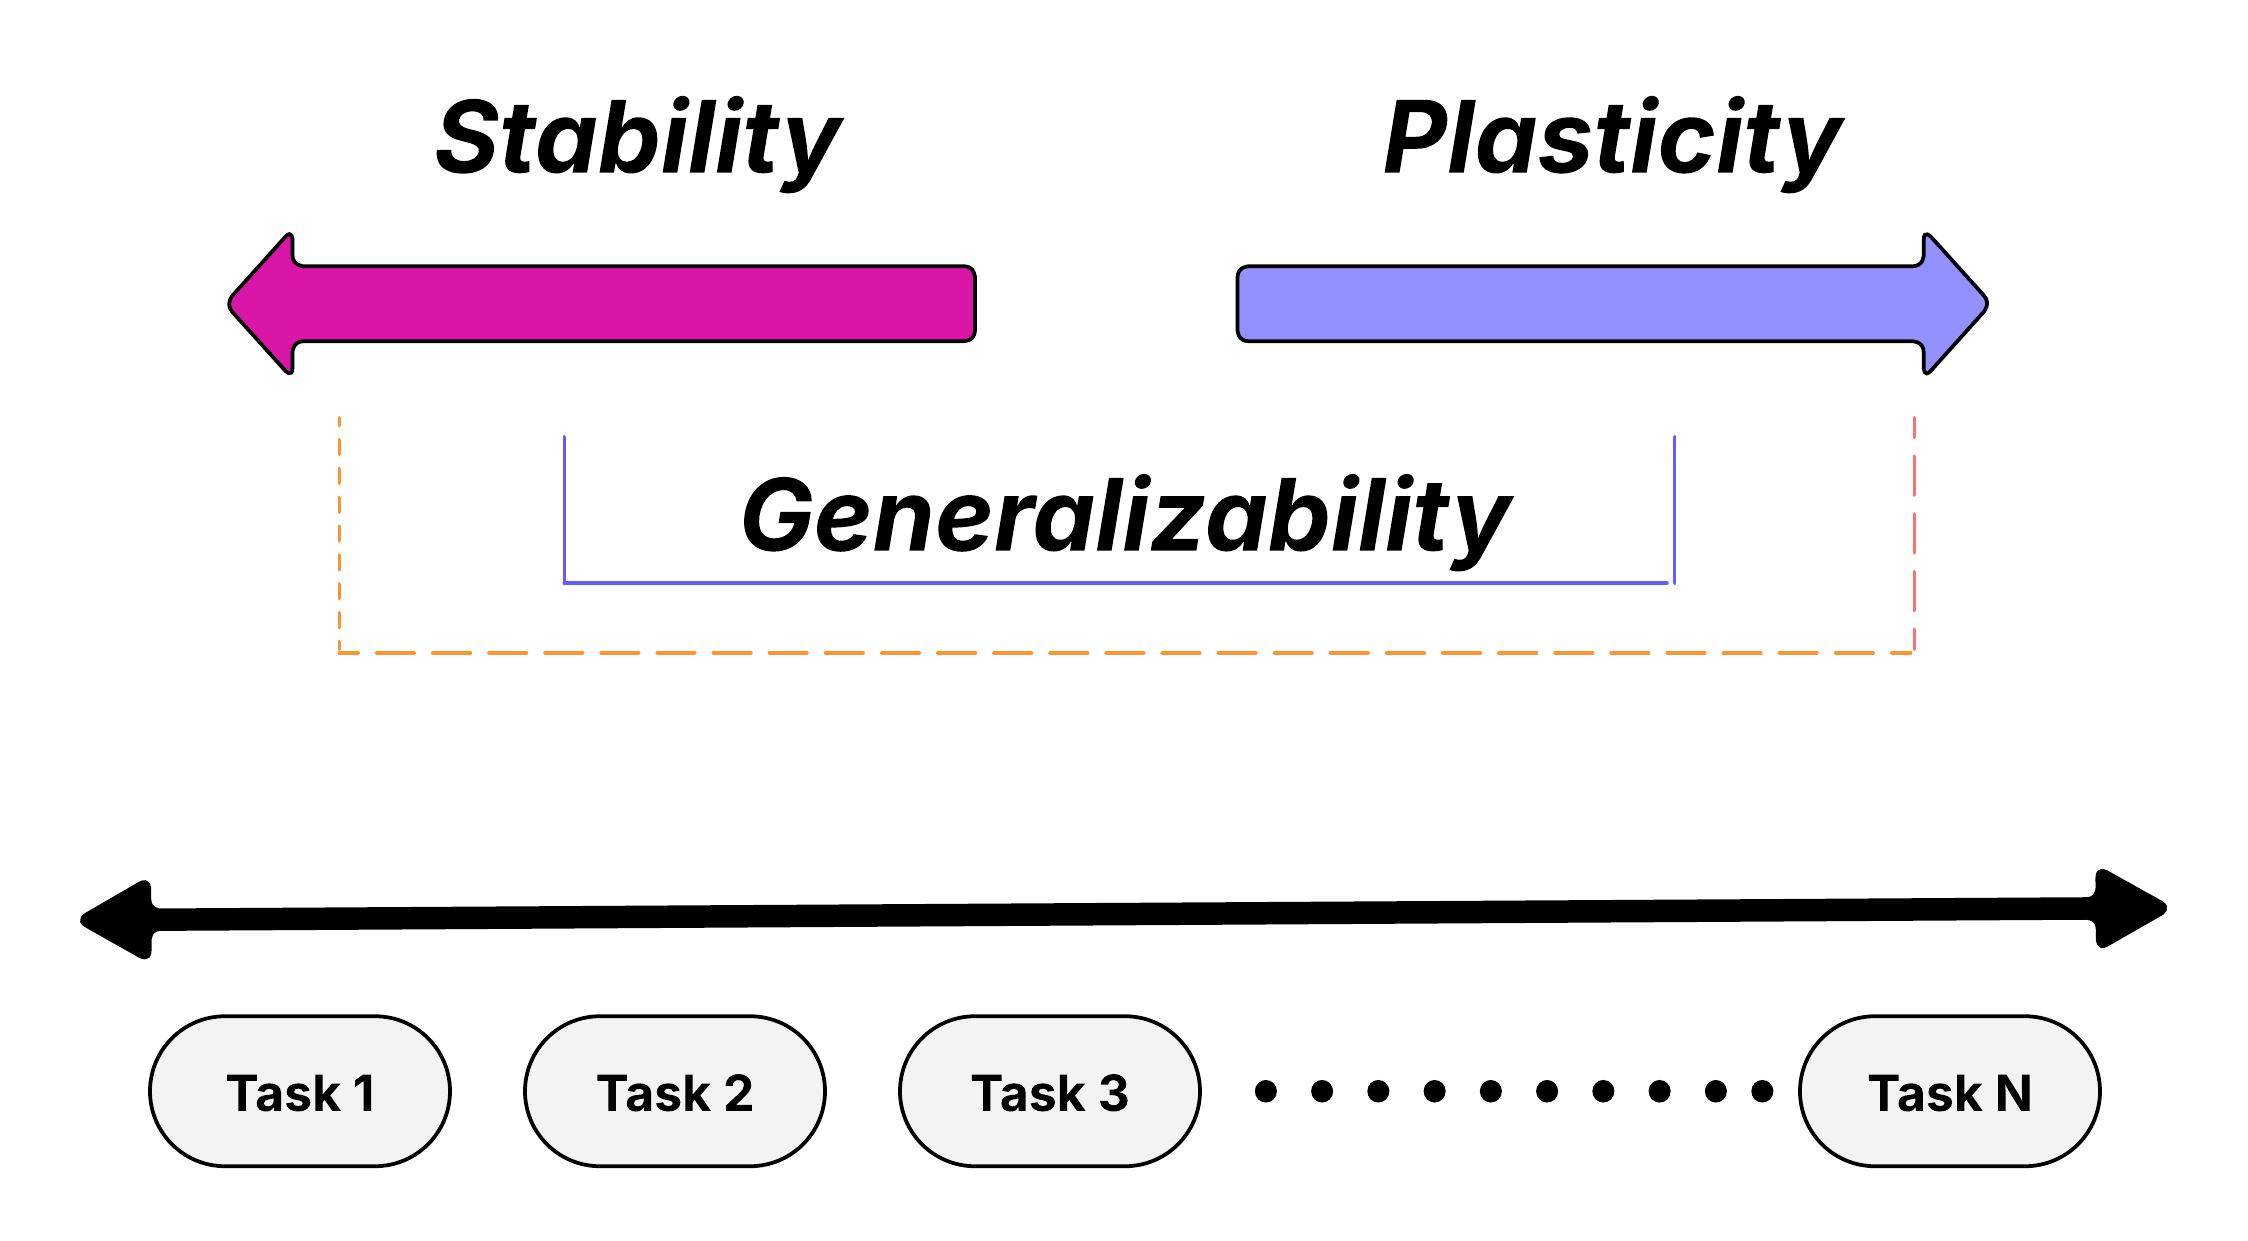
\includegraphics[width=\textwidth]{stabilityPlasticity.png}
    \caption{Illustration of the stability-plasticity dilemma in CL}
    \label{fig:stabilityPlasticity}
\end{figure}

From the optimization perspective, learning task t involves the application of gradient updates of the following form:

\begin{equation}
    \theta_t=\theta_{\left(t-1\right)}-\eta\nabla_\theta\mathcal{L}_t\left(\theta_{\left(t-1\right)}\right),\ 
\end{equation}

 where $\mathcal{L}_t(\theta)$ is the loss that needs to be minimized on the current task and $\eta$ is the learning rate.
This update might raise the loss  $\mathcal{L}_k(\theta)$  for some previously learnt tasks $k<t$, even when it increases performance on task $t$. Therefore, while excessive stability hinders successful adaptation to new activities, excessive flexibility causes forgetting. 
The model must update its parameters to integrate new knowledge while maintaining functionally significant parts of the parameter space. This limited optimization challenge is reflected in the stability–plasticity problem. By limiting parameter updates, replaying previous information, or assigning more model capacity, the majority of CL algorithms can be understood as means for controlling this trade-off\cite{6}.

\section{Catastrophic Forgetting}
One of the most challenging problem in CL is catastrophic forgetting, which occurs when a model trained on new tasks, it may rapidly drop performance on already learned tasks. Figure \ref{fig:CFillustration} illustrates that, as training progresses from one task to the next, performance on previously learned tasks degrades, while accuracy on the current task improves.

Weights that were significant for previous tasks may be overwritten by the gradient-based updates that neural networks rely on when the latest task data is added\cite{1}\cite{14}. As a result, even when the model has learnt the new task successfully, performance on previous tasks suffers. In sequential task learning, where tasks are presented one after the other without going over prior information again, catastrophic forgetting is very severe. In formal terms, if a model learns tasks $T_1,T_2,\ldots.,T_n$, the performance $A_i^j$ on task $T_i$ following training on task $T_j$ may fall as $j>i$, emphasising the need of techniques that maintain prior knowledge.
The standard metric\cite{20} for measuring forgetting is defined as:

\begin{equation}
    F_i=max_{l\in\{1,\ldots,t-1\}}A_i^l-A_i^t
\end{equation}

where $A_i^n$ is the accuracy on task $i$ after completing all $n$ tasks, $A_i^l$ is the accuracy on task $i$ after learning task $l$, and $F_i$ is the forgetting on task $i$. It is important to understand this equation because it shows the level of information learned in the past that is forgotten when learning new information.

\begin{figure}[!htbp]
    \centering
    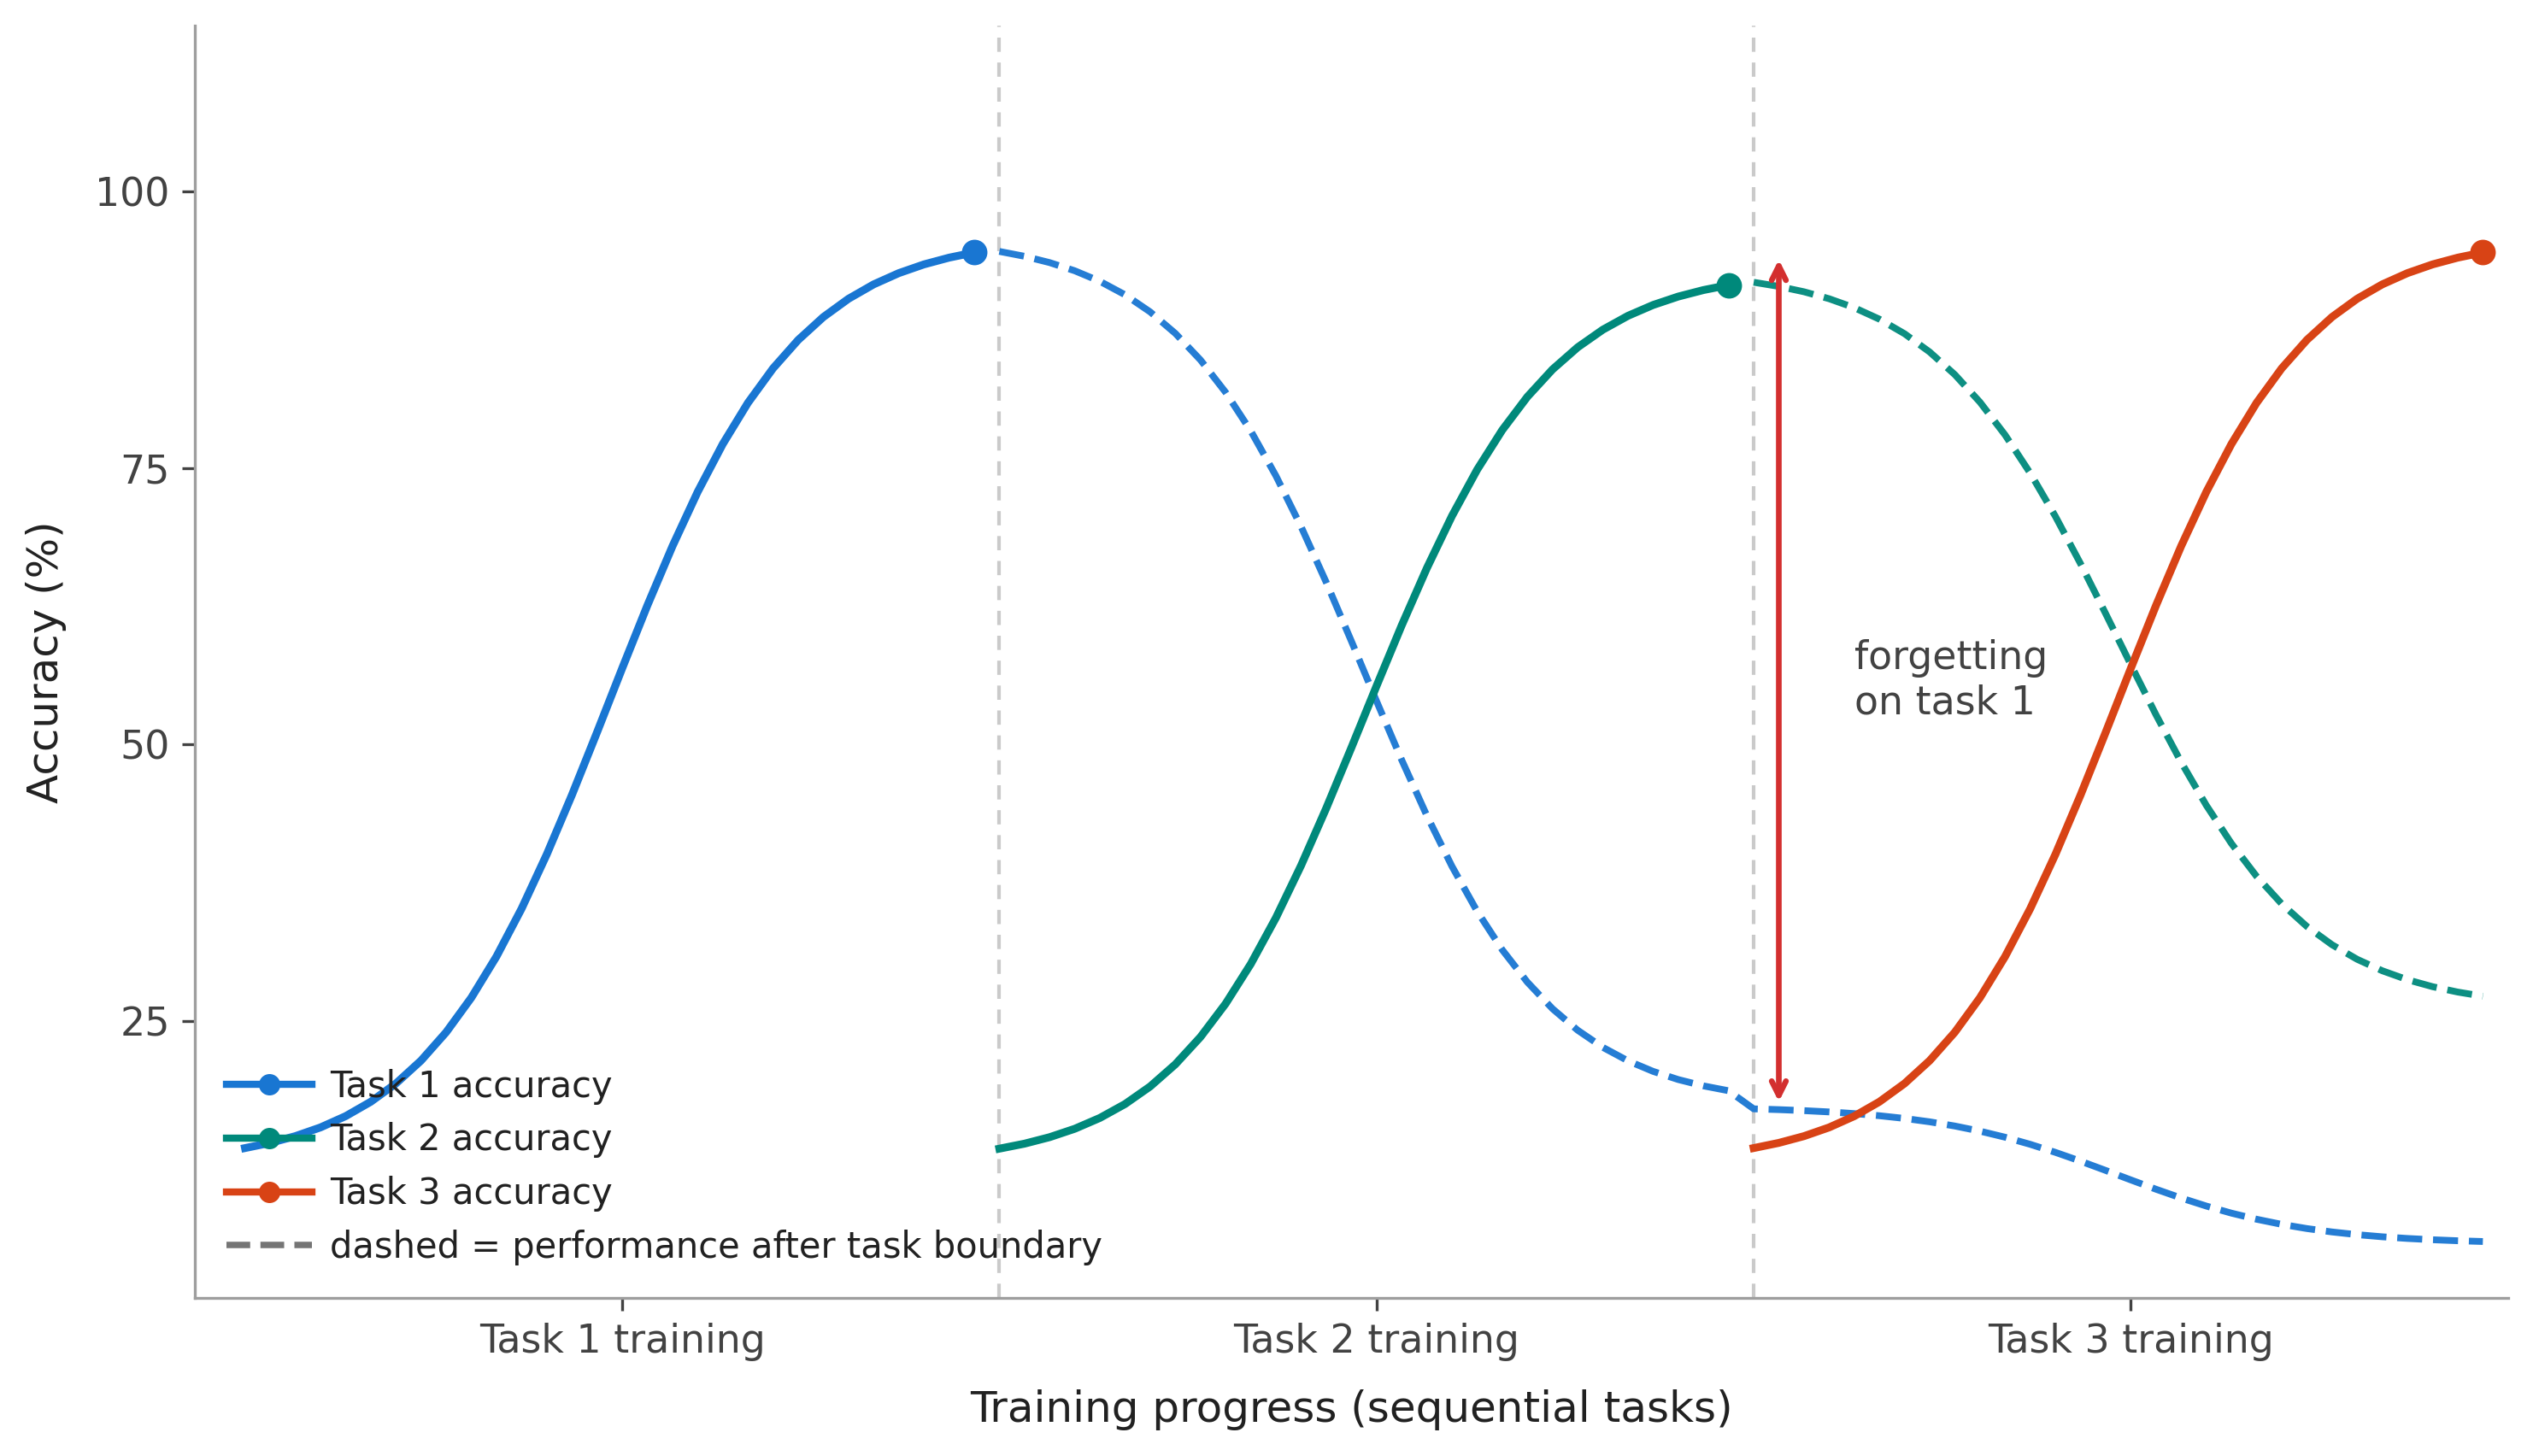
\includegraphics[width=\textwidth]{CFillustration.png}
    \caption{Schematic illustration of catastrophic forgetting in sequential task learning.}
    \label{fig:CFillustration}
\end{figure}

It is also important to understand the quantification of forgetting because it directs the designing of CL techniques\cite{6}, such as regularization, replay, and architectural techniques in an effort to strike a balance between learning and remembering.

\section{CL Evaluation Metrics}
Knowledge retention, task interaction over time, and prediction performance are important metrics that should be considered in the evaluation of CL systems. Performance is recorded at each level because the model is trained in a step-by-step manner over tasks $T_1,\ldots..,T_T$. After the model has been trained on task $T_j$, we define $A_i^j$ to be the accuracy on task $T_i$.
The average accuracy\cite{20} after learning every task is one important metric and is given by:

\begin{equation}
    Average\ Accuracy\ =\ \frac{1}{T}\sum_{i=1}^{T}A_i^T
\end{equation}

where $A_i^T$ is the accuracy on task $i$ after learning all tasks $T$. This metric does not measure forgetting in any way but gives a general overview of how well the model is performing.
For task $i$, forgetting is given by

\begin{equation}
    F_i = \max_{l\in{1,\ldots,T-1}} \left(A_i^l- A_i^T\right)
\end{equation}

This is the difference between the final accuracy on task i after learning all tasks and the maximum accuracy over task i during training.
The formula for calculating the average forgetting\cite{20} over tasks is: 

\begin{equation}
    F_{avg}=\frac{1}{T-1}\sum_{i=1}^{T-1}F_i
\end{equation}

The task interaction metrics offer further insights, apart from the aspect of forgetting. For example, the influence of learning new tasks on tasks that have already been learnt is given by the BWT\cite{20} metric: 

\begin{equation}
    BWT=\frac{1}{T-1}\sum_{i=1}^{T-1}\left(A_i^T-A_i^i\right)
\end{equation}

If the BWT metric is positive, the learning of new tasks will improve the performance of tasks that have already been learnt. If the BWT metric is negative, forgetting occurs.
The influence that tasks that have already been learnt will have on the upcoming tasks before they are learnt is given by the Forward Transfer (FWT)\cite{20} metric. This can be expressed as shown below:

\begin{equation}
    FWT=\frac{1}{T-1}\sum_{i=2}^{T}\left(A_i^{i-1}-b_i\right)
\end{equation}

This indicates the baseline performance on task $i$ before any training which can be expressed as $b_i$. In addition to the above task interaction metrics, the CL systems can be evaluated on other factors which include memory utilization, computational complexity, and model growth\cite{6}.  When combined, these metrics offer a thorough framework for evaluating CL model's overall effectiveness, stability, and flexibility.

\section{CL Strategies}
CL is meant to preserve performance on already learned tasks while training models on a series of tasks. Several kinds of techniques have been developed to treat catastrophic forgetting. These methods can be roughly classified into four categories: regularization-based methods, replay-based methods, dynamic architectural methods, and hybrid methods\cite{6}. They differ in how they preserve prior information. A specific approach to the stability-plasticity trade-off is provided by each category.

\begin{table}[h]
\centering
\caption{Categories of CL methods.}
\label{tab:cl_method_categories}
\small
\setlength{\tabcolsep}{3pt}
\renewcommand{\arraystretch}{1.25}
\begin{tabular*}{\textwidth}{@{\extracolsep{\fill}}p{2.4cm} p{3cm} p{2.8cm} p{2.4cm} p{1.8cm}@{}}
\toprule
\textbf{Category} & \textbf{Key Idea} & \textbf{Examples} & \textbf{Pros} & \textbf{Cons} \\
\midrule
Regularization &
Penalise important parameter changes &
EWC\cite{2}, MAS\cite{7}, LwF\cite{8} &
No data storage &
May limit plasticity \\
\addlinespace
Replay &
Store/generate past samples &
iCaRL\cite{9}, MeRGAN\cite{10} &
Strong retention &
Memory overhead \\
\addlinespace
Architectural &
Expand or isolate model structure &
DyTox\cite{11}, PNN\cite{22} &
No interference &
Model grows \\
\addlinespace
Hybrid &
Combine multiple strategies &
CL-DETR\cite{12}, iCaRL\cite{9} &
Best of both &
Complex \\
\bottomrule
\end{tabular*}
\end{table}

\subsection{Regularization-Based Methods}
Regulation of the parameter updates in the training of new tasks is the primary goal of the regularization-based methods, which try to preserve the previously obtained knowledge\cite{2}. These methods use a penalty term in the loss function to avoid large changes in key parameters. The general form of the objective function is given by:

\begin{equation}
    L_{total}=L_t+\lambda\Omega\left(\theta\right)
\end{equation}

where $\lambda$ is a regulating factor, $\Omega\left(\theta\right)$ is a regulating factor that depends on the deviation of the parameters from the previously learned ones, and $L_t$ is the loss function of the current task.

\subsubsection{Weight Regularization}
Weight regularization techniques penalize changes based on an estimation of each parameter's significance for prior tasks. EWC (EWC)\cite{2} is a prime example, in which the Fisher Information Matrix is used to approximate parameter importance. The loss is as follows: 

\begin{equation}
    L_{total}=L_t+\frac{\lambda}{2}\sum_{i}{F_i\left(\theta_i-\theta_i^\ast\right)^2}
\end{equation}

where $F_i$ indicates the significance of the parameters, and $\theta_i^\ast$ are the parameters following the previous task. During training for new tasks, this formulation prevents important parameters from drifting drastically. Similarly, Memory Aware Synapses (MAS) \cite{7} estimates parameter importance using the sensitivity of the model's output to parameter changes, rather than the loss, offering an unsupervised alternative to EWC.

\subsubsection{Functional Regularization}
Instead of preserving specific parameters, functional regularization techniques maintain the model's output behavior. Usually, knowledge distillation\cite{8} is used to accomplish this. Using a distillation loss stated as, 

\begin{equation}
    L_{distill}=\sum_{x}{\parallel f_{new}\left(x\right)-f_{old}\left(x\right)\parallel^2}
\end{equation}

The current model is trained to match the predictions of a prior model (teacher). This guarantees that predictions on prior tasks stay constant even if internal parameters vary.

\subsection{Replay-Based Methods}
By using data samples from past tasks during training, replay-based methods prevent forgetting. This is done without relying on constraints alone.
\subsubsection{Experience Replay}
Some real samples from past tasks are stored in a buffer during experience replay. During training on a new task, batches contain a mix of stored samples and the latest samples. The objective is:

\begin{equation}
    L_{total}=L_{current}+L_{replay}
\end{equation}

This training with a mix of samples stabilizes the representations and reduces the drift in parameters. For storing a representative mix of samples, techniques such as herding and reservoir sampling\cite{21} are often employed.

\subsubsection{Generative Replay}
By using a generative model $G\left(z,y\right)$ to fit the prior task distributions, the need for storing data is minimized\cite{10}. Then, the generated samples are created and utilized for training. This approach is highly dependent on the quality and semantic consistency of the generated samples, which is still challenging for complex vision tasks. Feature-level replay is a lightweight version of the method where the stored data is the intermediate representation, such as class prototypes.
\subsection{Dynamic Architectural Methods}
As a way of minimizing the interference between tasks, the dynamic architectures modify the structure of the model. In this approach, more memory is allocated or the routing mechanisms are adjusted based on the change of the tasks, unlike the constraints of the parameters or the reuse of the data.

Expansion of the networks enables the development of task-specific representations through expansion, which occurs through the addition of new neurons based on the tasks. This increases the size of the model, reducing the overlap of the tasks.

Dynamic approaches often involve the addition of task-specific tokens or modules to transformer-based models while maintaining a common backbone\cite{11}. For example, in order to add task-specific representations without retraining the model, new tasks tokens may be added to the input sequence.

In general, dynamic architectures can be considered to be learning a task-dependent function as follows:

\begin{equation}
    f(x;t;\theta_t)
\end{equation}

Here, a portion of the parameter set $\theta_t$ is task-specific to task $t$. Even though these approaches often achieve good results, they could potentially lead to increased costs in the future.

\subsection{Hybrid Methods}
For better balance between stability and plasticity, hybrid approaches combine elements from multiple categories. For example, distillation and replay\cite{9} can be combined in the following manner:

\begin{equation}
    L_{total}=L_{current}+L_{replay}+{\beta L}_{distill}
\end{equation}

For better retention, these formulations utilize both output constraints and data storage.

The latest approaches to vision models also combine replay and distillation with prompt tweaking or adapter components\cite{5}. In these cases, small components may adapt to new tasks while the underlying network is largely frozen\cite{22}. This minimizes parameter additions and forgetting.
Hybrid approaches are now being used in large-scale vision systems to better handle long and complex task sequences\cite{12}. These approaches aim to improve over single-strategy approaches in terms of scalability and robustness.

\section{Conclusions}
The theoretical background of CL and the key issues associated with sequential task training were presented in this chapter. The key drawback associated with conventional DL models under non-stationary conditions was identified as catastrophic forgetting. The fundamental challenge associated with knowledge retention and adapting to new tasks was described through the stability-plasticity trade-off.
Common metrics such as average accuracy, forgetting, FWT, and BWT were established with the aim of evaluating CL systems. These metrics were developed with the aim of creating a systematic approach for evaluating knowledge retention and flexibility. Issues such as memory usage and computational costs were also emphasized, especially for vision-based applications where task sequences may be long and complex.
The popular strategies for CL such as the regularization-based approach, the replay-based approach, the dynamic architectures approach, and the hybrid approach have also been covered in the chapter. It is important to remember that every strategy addresses catastrophic forgetting in a different way. For instance, the regularization-based strategy updates the rules governing the parameters, the replay approach revisits previously observed data, the dynamic architectures approach uses the architecture itself, and the hybrid approach combines all of these methods.
All of the above mentioned provide the background information needed to fully understand the techniques addressed and presented in the remainder of this work.

\chapter{Deep Learning Models for Vision}
\label{chap:3}
The DL architectures upon which the proposed approach is based are discussed in this chapter. It is important to understand the characteristics since it has a direct effect on how catastrophic forgetting occurs and how it can be alleviated.

Section \ref{sec:3.1} provides an introduction to the chapter. CNNs are discussed in Section \ref{sec:3.2}, with ResNet used as the CNN baseline for experimental comparison with other architectures. The ViT architecture, including how it uses patch tokenization and self-attention, and how pre-training plays a role in CL, is discussed in Section \ref{sec:3.3}. The concept of adapters, which are plugged into a frozen ViT architecture to facilitate task learning with few changes to the weights, is discussed in Section \ref{sec:3.4}. Section \ref{sec:3.5} introduces EWC in detail, which protects important adapter parameters using Fisher Information. Section \ref{sec:3.6} concludes the chapter and introduces how it relates to the system architecture in \hyperref[chap:4]{Chapter~\ref*{chap:4}}.

\section{Introduction}
\label{sec:3.1}
The fundamental architecture of a DL model has a significant impact on how likely it is to learn and remember visual information. Different architectural designs make different assumptions about how information should be contained within parameters, how features should be obtained, and how the model must respond to new data. These aspects directly affect how successfully a model may be modified for CL and how vulnerable it is to catastrophic forgetting.

CNNs have long been the preferred option for CV tasks. Their architecture, which is based on hierarchical feature extraction and local filters, performs well for images and has yielded impressive results on numerous benchmarks. However, new gradient updates frequently replace weights that were crucial for previous tasks when CNNs are trained sequentially on numerous tasks, resulting in severe forgetting.

An alternative is provided by ViTs, where images are divided into fixed-size patches, with each patch acting as a token, and self-attention is used to extract relationships in the entire image, rather than relying on local convolutions. ViTs provide rich and general feature representations when pre-trained on large datasets. ViTs are a suitable choice for CL environments where it is important to retain prior knowledge.

However, it is expensive and has the disadvantage that, in order to fully fine-tune a pre-trained ViT for a given task, there is a risk of disrupting the pre-trained representations. The solution is provided by adapter modules, where small trainable components are added to a frozen ViT backbone. Only the adapter's weights are updated during task training, and the overall model is left unchanged. This makes the learning process more efficient and reduces the risk of overwriting previously learned information.

The system suggested in this thesis work is built upon these architectural elements. Understanding how CNNs and ViTs store and update knowledge differently, as well as how adapters can be used to regulate parameter changes, is crucial to comprehending why the suggested method reduces forgetting. Each of these elements is covered in detail in the sections that follow.

\section{Convolutional Neural Networks}
\label{sec:3.2}
CNNs have been the leading models in the field of computer vision for a considerable number of years. This is because of the outstanding performance of CNNs in tasks like image segmentation, object detection, and image classification. In this section, the basic components of CNNs, the design principles, and the ResNet model, which is a basic model, are discussed. In the next section, the basic challenges CNNs face when dealing with problems related to CL, in which the tasks are sequential and the network is required to have prior knowledge of the tasks, are discussed.
\subsection{Architecture and Inductive Biases}
By creating models that closely resembles how images actually work, CNNs transformed CV. CNNs make assumptions to assist them comprehend how images work rather than treating each pixel as an independent unit as fully connected networks do.
Using a number of filters to analyse an image for patterns is the fundamental notion behind a CNN. A CNN creates an output $Y \in \mathbb{R}^{H' \times W' \times C'}$ by applying a filter $W \in \mathbb{R}^{k \times k \times C \times C'}$ to an input $X \in \mathbb{R}^{H \times W \times C}$,where $X$ is the input tensor, which can be an image, and $H$ and $W$ represent the height and width of the image, respectively. The number of channels of the input, denoted as $C$, can be 3 for a colored image.  The filter $W$ has a spatial size of $k\times k$, operates across all C input channels, and contains $C'$ individual filters each learning a different pattern. The resulting output $Y$ is a feature map of spatial dimensions $H'\times W'$ (determined by the stride and padding used) with $C'$ channels, one for each learned filter. 

CNNs are able to attain three essential properties thanks to this straightforward idea\cite{13}:
\subsubsection{Local connectivity}
Only a small portion of the input (with kernel size $k$) is connected to each unit. Since we can see an edge without seeing the full image it is a fair assumption in CV. A fully linked layer on 224x224 images has 50,176 weights per channel, while a $3\times 3$ kernel only has 9.
\subsubsection{Weight sharing}
The whole image is shared by the same filter. If we can spot vertical edges in one place, then we can use this detector anywhere in the image. Translation equivariance is achieved if a shift is made to the image, then a shift is made to the output. Weight sharing not only generalises well, but it also reduces parameters dramatically.
\subsubsection{Hierarchical features}
More complexity is introduced with multiple convolutional layers stacked together. Simple features such as corners and edges are found by the early convolutional layers. These simple features are then combined to form shapes, textures, parts of, or even whole objects by later convolutional layers. The receptive field is expanded, allowing each layer to see more of the original image. This is similar to how our brains process visual information, i.e., how our cortex is wired \cite{23}.

CNNs also downsample feature maps using pooling layers, usually max-pooling. This makes the network somewhat robust to little changes in the input by reducing the spatial size while retaining the crucial information. Convolution blocks (conv → batch norm → ReLU → pooling) with decreasing spatial size but growing feature channels alternate in the conventional architecture\cite{24}.
When the assumptions align with the problem, as they do with natural images, this architecture performs incredibly well. However, these same architectural decisions lead to particular difficulties in CL, which is addressed in Section \ref{sec:3.2.3}.

\subsection{ResNet and Skip Connections}
As CNNs became deeper to learn more complicated representations, an absurd problem emerged, very deep networks frequently performed worse than shallower ones, even on training data. Vanishing gradient problem started emerging when backpropagating through several layers, making it difficult to train the early layers successfully\cite{25}. This degradation issue was not caused by overfitting, but instead by optimization challenges.

To resolve this problem, He et al.\cite{3} introduced Residual Networks, where skip connections are used. This is a simple yet effective change to the neural network. ResNet blocks learn a residual function $F(x)$ and add it directly to the input, instead of learning a straightforward mapping $H(x)$ from input $x$ directly to output $y$:

\begin{equation}
    y = F(x) + x
\end{equation}

There are major consequences for gradient flow from this reformulation. Gradients can pass straight through the skip connection during backpropagation, bypassing the weights of the residual function. The skip connection guarantees that gradients still reach earlier layers even if $F(x)$ contributes little gradient (because of vanishing activations). This makes it possible to train networks with 50, 101, or even 152 layers, depths that were not achievable with simple CNNs.
Usually, two or three convolutional layers with batch normalization and ReLU activation functions are used to define the residual function $F(x)$. Each residual block in ResNet-18 and ResNet-34 models contains two $3\times3$ convolutional operations:

\begin{equation}
    F(x) = \mathrm{Conv}_{3\times3} \Big( \mathrm{ReLU} \big( \mathrm{BN} \big( \mathrm{Conv}_{3\times3}(x) \big) \big) \Big)
\end{equation}

The skip connection is just an identity mapping in which the input and output dimensions are the same. A 1x1 convolution is used to map the input to appropriate dimensions in case of dimension change due to spatial down sampling or increase in channels.

\subsubsection{ResNet-18 Architecture}
The 18 weight layers in ResNet-18 are divided into five stages. First comes a $7\times7$  convolution with a stride of 2, followed by $3\times3$ max pool. Then there are four stages with multiple residual blocks each, followed by a stride of 2 in each stage except stage 1\cite{3}. The structure is as follows:

\begin{itemize}
    \item Stage 1: $7\times7$ conv, 64 filters, stride 2 → $3\times3$ max pool
    \item Stage 2: $2\times$ residual blocks, 64 filters (output: $56\times56\times64$)
    \item Stage 3: $2\times$ residual blocks, 128 filters, first block stride 2 (output: $28\times28\times128$)
    \item Stage 4: $2\times$ residual blocks, 256 filters, first block stride 2 (output: $14\times14\times256$)
    \item Stage 5: $2\times$ residual blocks, 512 filters, first block stride 2 (output: $7\times7\times512$)
    \item Global average pooling → fully connected layer for classification
\end{itemize}
This gives us a relatively low 11.2 million parameters compared to ResNet-50 with 25.6 million parameters and ResNet-101 with 44.5 million parameters.

\subsubsection{Why ResNet-18 as a Baseline}
For a number of reasons, ResNet-18 is the baseline model. First of all, it embodies the conventional CNN methodology that dominated CV prior to the transformer era, knowing how it fails in CL inspires to investigate alternate designs. Second, ResNet-18 is typical of contemporary CNN design ideas and small enough to train effectively on Split CIFAR-100 with little computation. Third, the results are directly comparable to earlier studies because ResNet has been thoroughly investigated in CL literature. Lastly, when presenting adapter-based approaches that add only 0.32M trainable parameters, ResNet-18's 11.2M parameters offer a helpful reference point.

Even though ResNet performs well on common image classification benchmarks, residual connections are unable to address the catastrophic forgetting issue in CL. Weights crucial for earlier tasks are still overwritten when learning new tasks, and the network continues to employ shared, distributed representations across all tasks. The study of ViTs with modular adapter components in later sections is motivated by this fundamental constraint.

\subsection{CNNs in CL}
\label{sec:3.2.3}
CNNs are excellent at learning visual representations from big datasets, but learning sequentially across several tasks presents fundamental issues. In CL environments, the same architectural features that make CNNs efficient for single-task learning like shared filters and distributed representations become disadvantages.

CNNs have the problem of catastrophic forgetting since the gradients update the network's weights while training a CNN again on a new task.  CNNs have distributed representations, where all the neurons in the network take part in the generation of a multitude of features. As a result, CNNs will inevitably forget the learned representations while training the network to fit a new task. 

The catastrophic forgetting problem is particularly serious in the highly distributed structure of traditional CNN architectures, such as ResNet\cite{14}, because one filter in an early layer may assist in the detection of edges that are useful for the detection of various objects and tasks. All objects from task $t$, that relied on the edge detectors, would be affected if the weights of that filter are modified during the training of task $t+1$. There is no mechanism in CNN architectures that preserves the previously learned knowledge during the acquisition of new inputs, in contrast to architectures that incorporate task-specific components.

The most significant cause is weight interference, gradients from the new task push weights in ways that interfere with the performance on earlier tasks. The interference is not prevented by any residual connections, as they help with gradient flow during initial training. Even with skip connections that facilitate gradient flow, the gradients update all common weights.

A number of solutions for CL aim to address this problem. As mentioned before, EWC\cite{2} and other regularization-based techniques detect significant weights for prior tasks and penalise modifications to them. Examples from prior tasks are stored and interpolated during training on new tasks using replay-based techniques. Separate capacity is allocated to each task using architecture-based techniques. However, as depicted in the baseline trials where ResNet-18 records an average forgetting of 69.17\% across five tasks, the naive application of these techniques to CNNs can provide limited alleviation from forgetting.

These drawbacks imply that architectural modifications beyond merely regularizing conventional CNNs are necessary for CL. Ideally, we want models that can increase capacity for new tasks while keeping previously learnt representations. This drives our investigation of ViTs with adapter modules in the sections that follow. These architectures offer a natural division between common and task-specific information by combining a frozen shared backbone with task-specific modular components.

\section{ViTs}
\label{sec:3.3}
It was shown in Section \ref{sec:3.2} that the distributed and entangled representations of CNNs cause catastrophic forgetting. ViTs, an alternate architecture that extends the Transformer concept from Natural Language Processing (NLP) to CV, is examined in this section. This section examines how ViT uses self-attention and patch-based tokenization to analyse images, and explain why its modular block structure is better for CL than conventional CNNs.
\subsection{From NLP to Vision: The Transformer Architecture}
When Vaswani et al.\cite{26} first developed the Transformer architecture for NLP, it completely altered the comprehension of sequence modelling. Transformers use self-attention processes to process elements of a sequence in parallel, in contrast to Recurrent Neural Networks (RNNs) that process inputs sequentially. The gradient flow issues that affected deep RNNs were resolved by this design decision, which also made it possible to scale to far bigger models and datasets.

Self-attention, an approach that computes representations of each element by paying attention to all other elements in the sequence is the main innovation\cite{26}. The transformer uses learnt linear projections to calculate three vectors for each token in a series of input tokens, query ($Q$), key ($K$), and value ($V$). By using scaled dot-product similarity to compare each query with all keys, attention weights are calculated. A probability distribution is then obtained by applying softmax. As mentioned below in equation~\ref{eq:3.3} , the result for every position is a weighted sum of all values.

\begin{equation}
    \mathrm{Attention}(Q, K, V) = \mathrm{softmax} \left( \frac{Q K^{T}}{\sqrt{d_k}} \right) V
    \label{eq:3.3}
\end{equation}

where $d_k$ is the dimensionality of the key vectors.This is accomplished in parallel by many different attention heads. This is enabled by the ability of the model to look at the information provided in many different subspaces of the representation due to the presence of the multi-head attention mechanism. This output is then projected back to the model's dimensions.

Transformers make use of position wise feed-forward networks and a number of different layers of the multi-head attention mechanism. This is followed by the application of a feed-forward network to each position individually. In deep networks, training is stabilized by residual connections and layer normalization. Furthermore, transformers lack an innate sense of position because attention spans the entire sequence. In order to provide information about token order, positional encodings must be added to the input embeddings.

The obvious question posed by the success of the Transformer architecture in NLP is could this approach be extended to vision? Unlike language, vision does not have a natural notion of sequence, and for reasonable image sizes, processing each pixel as a token would be computationally costly. This is because the complexity of self-attention grows quadratically with sequence length, and we have 150,528 values in an RGB $224\times224$ image, which is just too many. Transformers were either incorporated into CNN architectures or merely focused on limited areas of the image in early attempts to use them for vision\cite{27}.

With the availability of large amounts of data, Dosovitskiy et al.\cite{4} have demonstrated that pure Transformer models may perform as well as CNNs for image classification. Instead of using pixels, their ViT (ViT) method considers a picture as a series of patches. This patch-based tokenization makes self-attention computationally possible by significantly reducing sequence length while maintaining spatial information. The ViT's performance demonstrated that, provided enough training data is available, the inductive biases inherent in CNNs, local connectivity and translation equivariance are not strictly required. The Transformer's scalability and flexibility, which were first shown in NLP, naturally translate to vision.

\subsection{Patch Embedding and Tokenization}
ViTs use a straightforward yet efficient method to address the computational challenge of applying self-attention to images by splitting the image into fixed-size patches and handle each patch as a token\cite{4}. Suppose a ViT divides an input image of size $H \times W \times C$ (height, width, and channels) into a grid of $N$ patches, each of which has $P \times P$ pixels. The length of the sequence that the Transformer will handle is determined by the number of patches $ N = (H \times W) / P^2$.

For conventional ViT configurations with $224\times224$ images and $16\times16$ patches, this results in a sequence of N = 196 tokens, which is significantly less than the 50,176 pixels in the original image. A learnt embedding matrix is used to flatten each patch into a vector of dimension $P^2 \times C$, which is then linearly projected to the hidden dimension $d\_model$ of the model. Similar to word embeddings in NLP, this projection transfers the raw input (image patches) into a high-dimensional representation space so that the Transformer can analyse them.

ViT includes two unique components in addition to the patch embeddings. The sequence is first preceded by a learnable class token $[CLS]$\cite{28}. This token just serves to aggregate global information through the self-attention mechanism but it has no relationship to any picture patch. Similar to BERT's method in NLP, the final representation of the $[CLS]$ token is used for classification after going through every Transformer layer. Second, to preserve spatial information about each patch's origin in the original image, positional embeddings are appended to each patch embedding (including the class token). The self-attention mechanism would handle every patch as an unordered set in the absence of positional information.

ViT-Tiny, a smaller version intended for effective training and deployment, is used in the experiments in this thesis work. ViT-Tiny creates 196 patch tokens and one class token (a total of 197) by applying $16\times16$ patches on $224\times224$ images\cite{29}. Compared to ViT-Base (768) or ViT-Large (1024), the hidden dimension, $d\_model$ = 192, is significantly less. Each of the 12 Transformer encoder blocks in the model consists of three heads with 64 dimensions each for multi-head self-attention, followed by a feedforward network with a hidden dimension of 768 (4× the model dimension). Every sub-layer is preceded by layer normalization, and each operation is wrapped by residual connections. This leads to a total of about 5.85 million parameters\cite{29}.

ViT-Tiny achieves a balance between computational efficiency and model capacity. ViT-Tiny works well for our Split CIFAR-100 tests, where the input images are just $32\times32$ (upsampled to $224\times224$ for compatibility with pre-trained weights), but ViT-Base (86M parameters) and ViT-Large (304M parameters) perform better on large-scale datasets like ImageNet-21k\cite{4}. The smaller design exhibits the main characteristics needed to investigate, modularity via the Transformer block structure and compatibility with parameter-efficient fine-tuning techniques while training more quickly on constrained computation (Google Colab T4 GPU). The pre-trained ViT-Tiny weights provide a robust feature representation derived from ImageNet, which is used as a frozen backbone in this adapter-based approach.

\subsection{Self-Attention Mechanism}
The fundamental function that enables Transformers to model relationships between every point in a sequence at once is self-attention. Self-attention computes each output position as a weighted combination of all input locations, in contrast to convolution, which only links adjacent positions via local receptive fields. Because of its global connection, the model can capture long-range dependencies without being constrained by CNNs' depth.
Three learnt projections of the input are used by the process. Using learnt linear transformations, as stated before we calculate a query vector (q), a key vector (k), and a value vector (v) for every token in the sequence. The key stands for \enquote{what do I offer}, the query for \enquote{what am I looking for}, and the value for \enquote{what information do I carry}. We calculate the following for an input sequence $X \in \mathbb{R}^{N \times d\_{\text{model}}}$:

\begin{equation}
    Q = XW_Q,  K = XW_K,  V = XW_V
\end{equation}

where $W_Q, W_K, W_V \in \mathbb{R}^{(d\_model\times d_k)}$ are learned weight matrices.
The dot products are utilized in the calculation of the attention weights by comparing each of the queries with each of the keys. The level of attention that the token at position $i$ has for position $j$ is determined by the dot product $q \cdot k_i$. The attention weights are normalized by softmax, which generates a probability distribution after being scaled by $1/\sqrt d_k$, which prevents values from becoming too large and hence producing a nearly one-hot distribution:

\begin{equation}
    attention_{weights} = softmax(QK^T / \sqrt d_k)
\end{equation}

Using the attention weights as the coefficients, the final output for each position is determined by a weighted sum of all the value vectors. A high attention weight for positions $i$ and $j$ implies that a lot of information is incorporated at position $i$ from position $j$.

Transformers use several attention heads working in parallel instead of computing a single attention function which can be referred as multi-head attention\cite{26}. Each head computes attention individually and has its own set of learned projection matrices $(W_Q, W_K,$ and $W_V)$. ViT-Tiny employs three attention heads, each measuring 64, for a total model dimension of 192. Different heads learn to concentrate on different kinds of relationships. Some may focus on distant patches (recording global context), while others may focus on adjacent patches (learning local patterns akin to convolution). A final learnt matrix is created by concatenating the outputs from each head and projecting them back to $d\_model$.

The self-attention process in ViTs makes use of the class token as well as a series of image patches. Similar to the local receptive fields observed in CNNs, the early layers tend to display local attention patterns, where every patch primarily focuses on its spatial neighbors. However, the patches in the later layers tend to focus on semantically relevant areas of the entire image, as opposed to their spatial position, thereby displaying global attention patterns. In order to make the classification decision, the class token tends to focus on a large number of patches. In the context of CL, this flexibility in the learned attention patterns plays a significant role. Every transformer layer possesses distinct parameters, which can be separately frozen or tuned, as opposed to the filters in CNNs, which are shared by every spatial position. Architectural modifications, as discussed in the context of adapter modules in Section 3.4, are made possible.

\subsection{Pre-training and Transfer Learning}
One of the key findings of the original ViT paper\cite{4} is that pre-training is a key factor for improving ViTs. While the flexibility of the transformer architecture might be higher than that of CNNs, the latter need less data to learn efficient visual representations from scratch.  CNNs have a high inductive bias, including assumptions of spatial locality and equivariance. ViTs underperform ResNet architectures of similar sizes when they are only trained on ImageNet-1k, a dataset of 1.3 million images\cite{4}. 

However, ViTs achieve or beat CNNs when they are pre-trained on larger datasets, including ImageNet-21k, a dataset of 14 million images.
A fundamental trade-off between inductive bias and flexibility of models is represented through the data efficiency gap between ViTs and CNNs. CNNs incorporate presumptions about images, which allow efficient learning from scarce data, but might restrict the performance of CNNs. While ViTs might perform better if enough pre-training data is available, they make fewer presumptions than CNNs and need more data to find visual structure.

Replacing the classification head with a new randomly initialized layer and then fine-tuning the entire model is the conventional way of adapting a pre-trained ViT for a novel task\cite{30}. This works well for single-task learning, yet it causes difficulties in the context of CL, as changing all parameters for a novel task significantly changes the shared representations, thereby disrupting knowledge for prior tasks. The alternative is to treat the ViT as a pre-trained feature extractor by completely freezing the pre-trained backbone and then training the new head. This prevents adaptation to new task features, yet it prevents catastrophic forgetting in the backbone.

Using the timm library\cite{31} , we use a pre-trained ViT-Tiny, which has been pre-trained on ImageNet. 1.28 million natural images were utilized in learning this model's ability to perform a wide range of tasks. For Split CIFAR-100 experiments, we completely freeze these pre-trained weights, and for task-specific adaptation, we use lightweight adapter modules (Section 3.4). Although it is possible, with the lightweight adapter modules, to learn without interfering in any prior activities, completely freezing the weights ensures that the model retains its ability to perform a wide range of tasks.

\subsection{ViT vs CNN in CL}
CNNs and ViTs have different architectures. This offers different learning opportunities and challenges. CNNs have a catastrophic forgetting problem, as discussed in Section \ref{sec:3.2.3}. The single filter of an early layer is useful for edge detection, which is useful for many different object types for many different tasks. All previous tasks that relied on these edge features are affected when the filter is changed during learning on a new task. It is difficult to adapt the network for new knowledge without affecting previously learned knowledge, as knowledge is represented in a distributed and entangled manner.

However, ViTs propose an alternative framework for this problem, as information flows across all the blocks, and the modularity of the architecture allows for natural boundaries where interventions may be made\cite{4}\cite{5}. Each of the Transformer blocks processes information in different ways, as seen in the different layers of self-attention and feedforward layers. This is in contrast to the filters of a convolutional layer, which must be applied equally across all spatial positions, as the self-attention mechanism allows for the acquisition of attention patterns individually for different circumstances. Most importantly, the stacking of identical components in the Transformer architecture enables task-specific components to be incorporated systematically (e.g., through adapters).

\begin{table}[h]
\centering
\caption{CNN vs ViT comparison.}
\label{tab:cnn_vit_comparison}
\small
\renewcommand{\arraystretch}{1.2}
\begin{tabular*}{\textwidth}{@{\extracolsep{\fill}}l l l@{}}
\toprule
\textbf{Property} & \textbf{CNN (ResNet-18)} & \textbf{ViT-Tiny} \\
\midrule
Feature extraction      & Local convolutions                & Global self-attention \\
Inductive bias         & High (locality, equivariance)    & Low \\
Parameters             & 11.2M                             & 5.85M \\
Pre-training data needed & Less                            & More \\
Modularity for CL      & Low                               & High \\
\bottomrule
\end{tabular*}
\end{table}

Modularity is the main advantage of CL, although additional components may be learned for task-specific adaptations, the frozen ViT ensures a stable task-agnostic visual representation. The problem of stability-plasticity is immediately solved by the division of knowledge into task-specific and shared knowledge. The model is flexible, as the adapters may pick up new patterns, and it is stable, as the basic representations are safeguarded.

However, ViT itself is not a complete method for CL, as it has been seen in the baseline experiments, where a naive fine-tuning of ViT-Tiny for sequential tasks leads to an average forgetting of 63.26\% and an average accuracy of 41.91\%. This is still a disaster, although it is slightly better than the performance of ResNet-18, which has an average forgetting of 69.17\% and an average accuracy of 24.22\%. The advantage of the modularity of the ViT, as well as architectural and regularization techniques specifically designed for the CL setting, is what our method leverages, which incorporates EWC for the protection of the critical parameters of the adapters (Section \ref{sec:3.5}), additional lightweight adapters for task-specific learning (Section \ref{sec:3.4}), and a frozen ViT backbone.

\section{Adapter Modules for Parameter-Efficient Learning}
\label{sec:3.4}
While ViTs provide modular design, comprehensive fine-tuning leads to catastrophic forgetting. Adapter modules, which are lightweight trainable parts added to frozen pre-trained models, are discussed in this section. By separating shared and task-specific knowledge, adapters facilitate task-specific learning while maintaining backbone representations, which is crucial for CL.
\subsection{Motivation: Parameter-Efficient Fine-Tuning (PEFT)}
In present day DL, fine-tuning huge pre-trained models on downstream tasks has become the norm. However, there are practical difficulties with changing every model parameter. To fine-tune a ViT-Base model with 86 million parameters, a full copy of each task's weights must be stored. This storage need becomes prohibitive in cases involving CL and several sequential tasks. More importantly, when all parameters are updated, there is a chance of catastrophic forgetting, which means that the model's representations for earlier tasks are erased as it adjusts to new input.

PEFT methods overcome these issues by introducing a limited set of extra trainable parameters, leaving the remainder of the pre-trained model frozen. However, the major breakthrough is that the pre-trained models often encode features that are relevant to a wide variety of tasks. We can derive a set of lightweight task-specific transformations to fine-tune the frozen features to each new task, instead of adapting these common features. This reduces storage space requirements by using one frozen model and a set of N small parameter sets, compared to using one set of parameters for each of the N models.

\begin{table}[h]
\centering
%\caption{PEFT methods comparison.}
\caption{Comparison of representative parameter-efficient fine-tuning (PEFT) methods.}
\label{tab:peft_methods_comparison}
\small
\setlength{\tabcolsep}{2pt}
\renewcommand{\arraystretch}{1.2}
\begin{tabular*}{\textwidth}{@{\extracolsep{\fill}}l l c l@{}}
\toprule
\textbf{Method} & \textbf{Approach} & \textbf{Params Added} & \textbf{CV Performance} \\
\midrule
Houlsby et al.\cite{15} & Bottleneck modules           & \textasciitilde0.5--3\% & Strong \\
AdaptFormer\cite{32}        & Post-attention adapters      & \textasciitilde1--2\%   & Matches full FT \\
LoRA\cite{34}               & Low-rank weight decomposition & \textasciitilde0.1--1\% & Strong in NLP \\
Prompt Tuning\cite{visualprompttuning}      & Learnable input tokens       & \textasciitilde0.01\%   & Task dependent \\
\bottomrule
\end{tabular*}
\end{table}

This method is exemplified by adapter modules, which were introduced for NLP by Houlsby et al.\cite{15}. A small neural network element added to a pre-trained model is called an adapter. Only the adapter parameters are modified during fine-tuning and the original model parameters stay unchanged. Without changing the underlying feature extractor, the adapter learns to modify the frozen model's representations for the new task. In order to achieve strong performance while updating less than 5\% of the total model parameters, many adapter designs employ bottleneck architectures with significantly fewer parameters than the layers they optimise.

The question of whether comparable methods may be effective for vision models was naturally sparked by the success of adapters in NLP (BERT, GPT)\cite{15}\cite{28}. Adapter-based fine-tuning for CV became possible with the development of ViTs, which have architectural similarities to language Transformers. Adapters can rival full fine-tuning performance on vision tasks using only a fraction of the trainable parameters, as several recent works \cite{32}\cite{chen2023visiontransformeradapterdense}\cite{visualprompttuning} have shown.

Beyond efficiency, PEFT approaches provide a strong advantage for CL which is modularity. A natural division between task-specific information (the adapters) and shared knowledge (the frozen features) can be achieved by freezing the pre-trained backbone and training distinct adapter sets for each task. The stability-plasticity problem is immediately addressed by this architectural division. Since the previous task knowledge cannot be removed, the frozen backbone provides a guarantee of stability. The model is still able to learn new patterns through the task-specific adapters. However, the adapters are insufficient to prevent catastrophic forgetting, as discussed in the following Section \ref{sec:3.4.4}. The adoption of regularization techniques like EWC is motivated by the fact that, even while the frozen backbone is safeguarded, the adapter parameters themselves may still experience interference when shared across numerous processes.

\subsection{Adapter Architecture}
As stated before, the common design pattern in parameter-efficient transfer learning is the adapter architecture in BERT fine-tuning, which was first demonstrated in Houlsby et al.\cite{15}. The general idea is to append small trainable modules to a pre-trained, frozen network, which enables the adaptation to a specific task without modifying the original parameters.

 

\begin{figure}[!htbp]
    \centering
    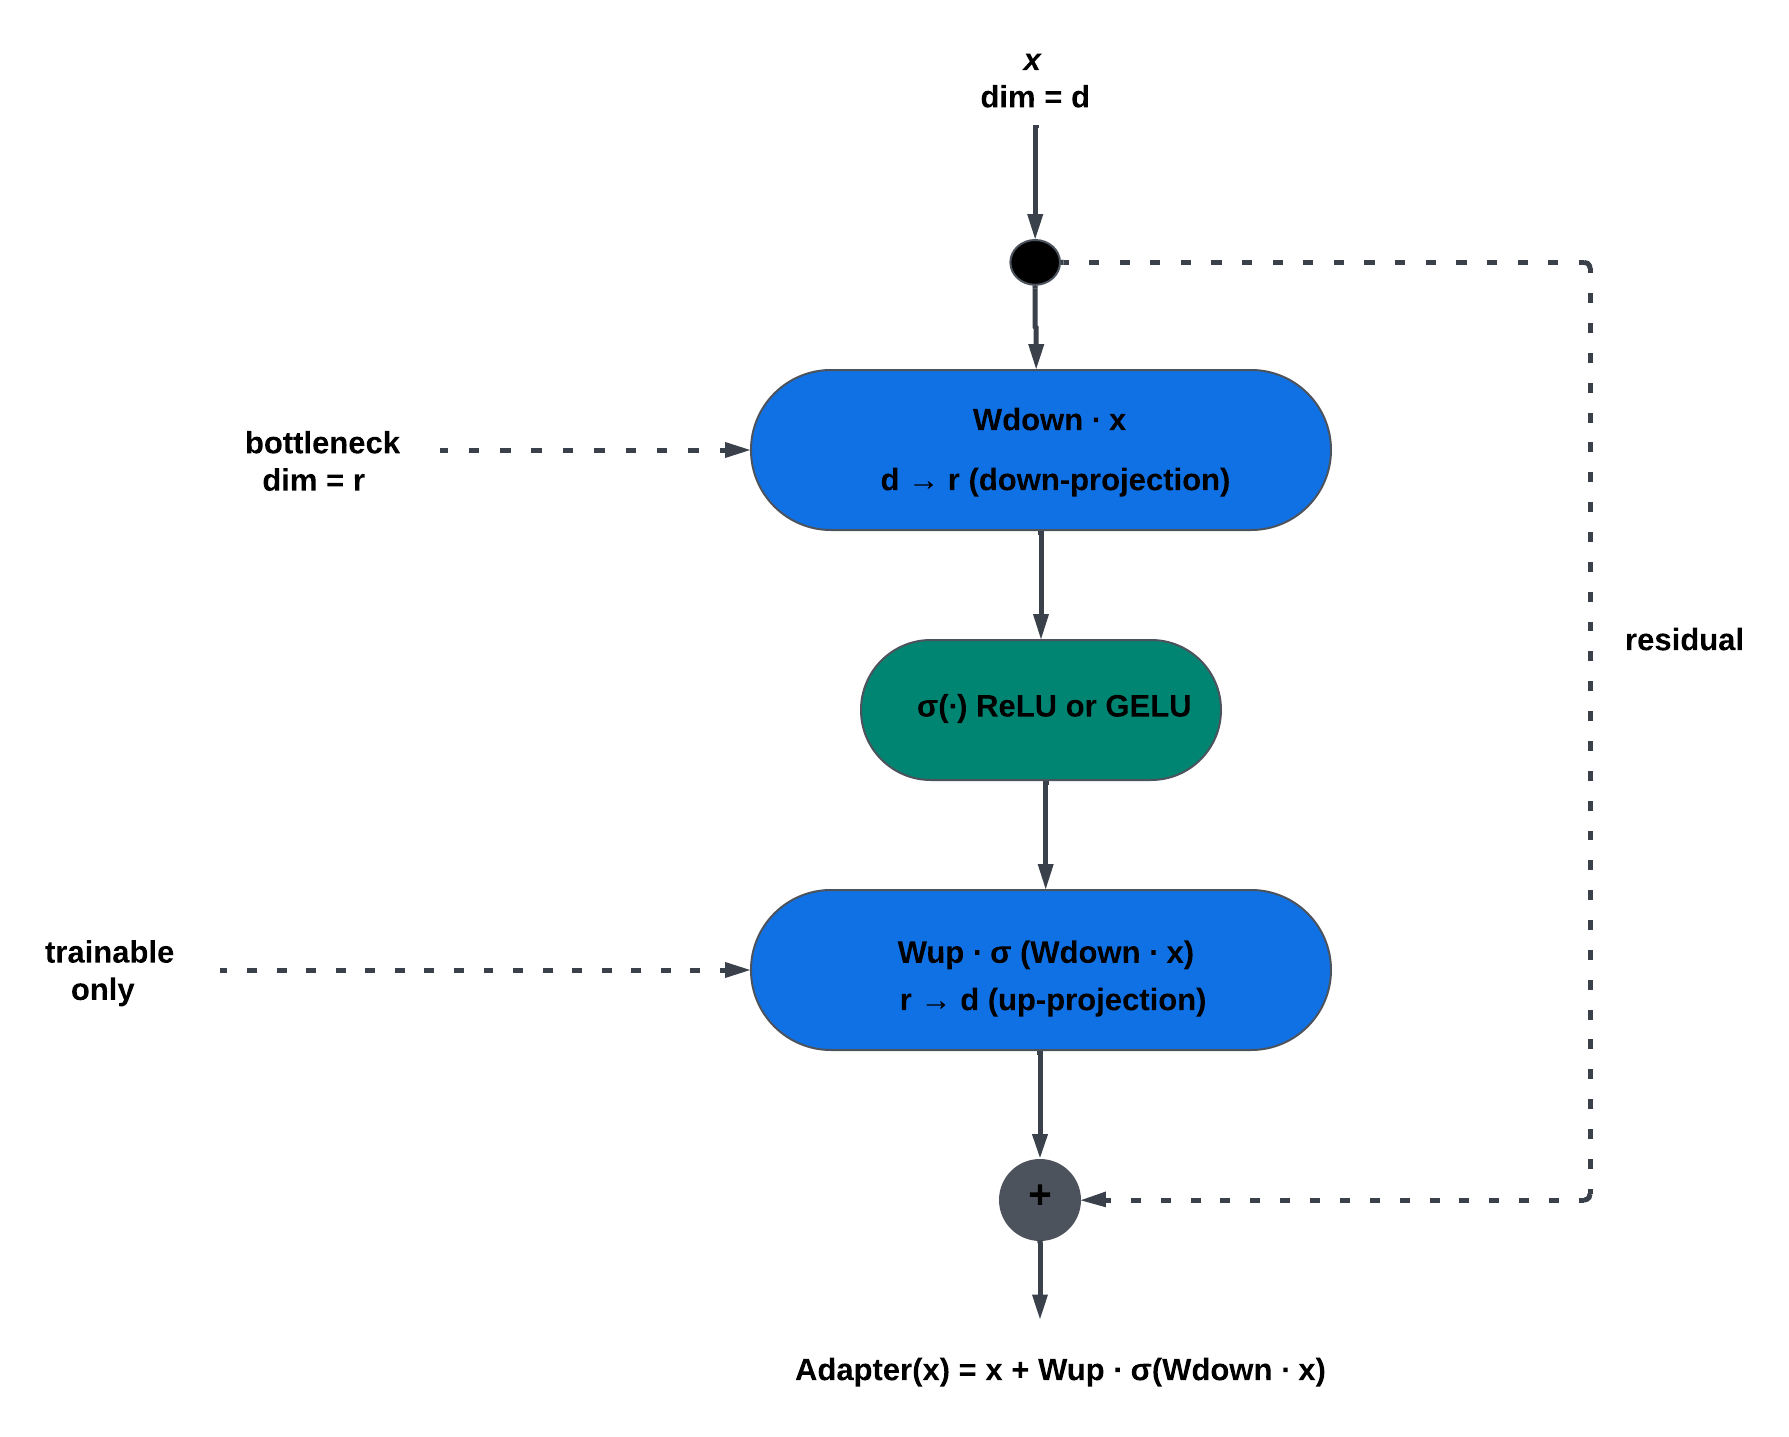
\includegraphics[width=\textwidth]{adapterarchitecture.png}
    \caption{Adapter architecture}
    \label{fig:adapterarchitecture}
\end{figure}

A bottleneck structure, which balances expressiveness and parameter efficiency, is a common trait in the majority of adapter architectures. Typically, an up-projection to the original dimension, a nonlinear activation function, and a down-projection layer, which reduces the dimensionality of the input, define a typical adapter module. If desired, a residual connection is used to ensure the ability to approximate the identity function:

\begin{equation}
    Adapter(x) = x + W_{up} \cdot \sigma(W_{down} \cdot x)
\end{equation}


where $\sigma$ is usually ReLU or GELU, $W_{down}$ maps from the model dimension $d$ to a bottleneck dimension $r$, and $W_{up}$ maps back to $d$. Note that, unlike the $O(d^2)$ parameters in a full layer, the dimension of the bottleneck is significantly smaller than the dimension of the model, adding only $O(2dr)$ parameters. Houlsby et al.\cite{15} found that reduction factors of $16-64$, or $r = d/16$ to $d/64$, were effective for the BERT model, although later work\cite{32} suggests that a reduction factor of 4-8 is sufficient for CV models. 

To avoid disturbing pre-trained representations, appropriate initialization of the adapter is crucial. $W_{up}$ is initialized near zero, as in Houlsby et al.'s work\cite{15}, so the adapter is initialized as an approximate identity and continues to learn useful transformations throughout the course of the training procedure. Lester et al.'s\cite{33} work proposes the use of one adapter per block, placed after the feed-forward sublayer in the Transformer architecture, and found this to be more effective than Houlsby et al.'s\cite{15} use of two adapters, one after the attention and one after the feed-forward, while still maintaining similar performance.

Adapter-based fine-tuning has naturally expanded to CV with the emergence of ViTs. Adapters match full fine-tuning on image classification while updating less than 2\% of parameters, as Chen et al.\cite{32} show. 
Similar results have been shown in the tasks of object detection and segmentation in Li et al.\cite{exploringplainvisiontransformer}. This shows that the techniques of bottleneck compression, residual connections, and initialization have a successful translation from the linguistic domain into the visual domain when using Transformer architectures.

However, single-task or multi-task learning with joint training is the main focus of existing research. There is still much to learn about the use of adapters in CL, where tasks are delivered one after the other. Although the flexibility of using adapters is a notable aspect, whereby the ability to differentiate between the task-specific, trainable parameters and the frozen backbone is utilised, as shown in the coming sections, this does not guarantee the phenomenon of catastrophic forgetting.
Other parameter-efficient approaches such as Low-Rank Adaptation (LoRA) \cite{34} have also shown strong results, decomposing weight updates into low-rank matrices as an alternative to bottleneck adapters.

\subsection{Adapters in CL}
\label{sec:3.4.3}
The architectural characteristics of the adapters make them particularly appealing for CL, although they were first developed for parameter-efficient transfer learning in single-task or multi-task settings. The primary advantage of the distinction between trainable task-specific parameters and frozen pre-trained parameters is the distinction itself. This distinction provides a natural way of retaining prior knowledge while allowing adaptation to a new task in a CL environment where tasks occur sequentially.

We maintain the general visual representations gained from ImageNet by maintaining the pre-trained ViT backbone frozen during sequential task training. These representations such as shape features, texture patterns, edge detectors, and semantic concepts act as a common feature space for all tasks. These parameters cannot be replaced by gradients from new tasks since they never update after the initial pre-training period. This completely removes catastrophic forgetting at the backbone level.

Thus, the trainable adapter modules ensure flexibility, whereas the frozen backbone ensures stability\cite{11}. In effect, each adapter is given the power to alter the frozen features in any way deemed necessary for the given problem at hand. For instance, the adapters can be trained to emphasize certain dimensions of the features that can be more discriminitive when differentiating between the object categories relevant to the problem at hand. The adapters can alter the frozen features without replacing them entirely because they do so through residual connections.

For managing adapters across various tasks in CL, there are a few techniques. Setting unique adapters for all tasks and keeping their weights unique to all tasks and only activating their respective sets during inference can be one technique. This technique offers maximum protection against forgetting. However, this technique demands knowledge of task identity during testing and also stores $N$ adapter sets for $N$ tasks (TIL). Another technique for managing adapters across all tasks in CL is to train adapters sequentially on all tasks. This technique can be more memory-friendly and can also be applicable to CIL when task identification is unknown during testing\cite{18}. However, there is a probability of adapter weight interference occurring due to fresh task training, which may override adapter weights that are essential for previous tasks.

The shared adapter method, which we use in our experiments, consists of the successive training of a single set of adapters for each of the five split CIFAR-100 tasks. This tests whether adapters, combined with the frozen backbone, help to mitigate forgetting even when the adapters’ parameters are shared. Our ViT model, combined with adapters, has an average accuracy of 76.93\% and an average forgetting score of 19.91\%, compared to 63.26\% and 69.17\% for the full ViT fine-tuning and the ResNet-18, respectively. This indicates a marked improvement over the baseline methods. The proposed architecture for adapters allows for the efficient learning of new tasks, and the frozen backbone provides robust protection.

Despite the fact that the 19.91\% forgetting is significantly better than the baselines, there is still a drop in performance. This implies that when the parameters of the adapter are sequentially modified across tasks, there is still interference, although significantly lower than the full model. There is a loss of task-specific information since the same weights used for the purpose of modifying the features of Task 1 are being used for the purpose of servicing Tasks 2, 3, etc. This limitation calls for the adoption of mechanisms that ensure the regularization of critical parameters of the adapter, as discussed in Section \ref{sec:3.5}.

\subsection{Limitations and Remaining Forgetting }
\label{sec:3.4.4}
The adapter-based model still demonstrates 19.91\% average forgetting over five tasks. While this represents a considerable drop from baseline approaches, as seen in the performance of ViT-Tiny (63.26\%) or ResNet-18 (69.17\%), this demonstrates that isolation, as a solution, is not sufficient to address CL.

The source of this residual forgetting is interference from the adapter's weights. While pre-trained knowledge is preserved through the frozen backbone, the adapter's parameters are shared and sequentially updated throughout tasks. When training for the second task, gradient descent adjusts the adapter's weights to optimize for reduced loss on new input, thereby affecting the first task's relevant representation. Even in the relatively small parameter space for the adapter, there is interference.
As the number of tasks increases, the degradation gets worse. This degradation might be caused by the utilization of parameters that are vital for Task 1 for Task 3. Adapters reduce interference when compared to comprehensive fine-tuning. However, they do not solve the stability-plasticity trade-off completely.

This restriction proves that the design of the architecture is not enough for successful CL. Even though adapters greatly reduce interference, vital parameters within this area need protection. In Section \ref{sec:3.5}, the EWC method, which uses architectural modularity together with parameter protection to reduce forgetting from 19.91\% to 2.01\%, is discussed.

\section{EWC}
\label{sec:3.5}
Even when the adapter-based method significantly outperforms baselines, adapter weight interference across tasks causes significant forgetting. This section presents EWC, a regularization method that penalises modifications to weights determined to be crucial for prior task performance in order to protect important parameters. 

\subsection{Regularization-Based CL}
The adapter-based method reduces catastrophic forgetting through the freezing of the pre-trained backbone network's weights and the training of task-specific parameters. However, as it was stated in Section \ref{sec:3.4.3} that weight interference among the shared adapter parameters contributes 19.91\% of catastrophic forgetting. In this work, the regularizer-based CL method is adopted, which avoids the overwriting of important parameters during the training of new tasks.

As explained before, regularization-based methods include penalty terms in the loss function that deter significant adjustments to parameters considered crucial for earlier tasks. The regularization technique works by constraining the optimization process. In contrast, the replay technique constrains the information used, whereas the architecture-based technique constrains the capacity of each task\cite{6}. However, the major challenge in the regularization technique is the identification of the parameters that are important. It should be safe enough to update the less important parameters since the weights of the tasks are not equally important.

One excellent method using the Bayesian principles is the EWC method, which was first proposed by Kirkpatrick et al.\cite{2}. The main idea is that the parameters $\theta$ represent a posterior distribution over the values that were most likely given the data after training on Task 1. The main idea is to find parameters that work well for Task 2 but still have values close to those that worked well for Task 1. This is achieved by the method by adding a quadratic penalty to the parameters based on their values for Task 1. The strength of the penalty is proportional to the importance of the parameter for Task 1.

\subsection{Fisher Information and Parameter Importance}
The Fisher Information Matrix is a concept from information theory that measures the sensitivity of the predictions made by the model to changes in the model's parameters. EWC uses the Fisher Information Matrix to measure the relevance of the parameters to the model\cite{2}. The predicted value of the square gradient of the log-likelihood with respect to the model's parameters $\theta_i$ is given by the Fisher information $F_i$:

\begin{equation}
    F_i = \mathbb{E} \left[ \left( \frac{\partial \log p(y \mid x, \theta)}{\partial \theta_i} \right)^2 \right]
\end{equation}

It makes sense to say that if the model predictions are heavily affected when $\theta_i$ is changed (big gradients), then $F_i$ is high, meaning the parameter is very important to the model. We can safely set the value of $\theta_i$ to different values when the model is to be applied to a different task if the predictions made by the model do not depend heavily on the value of $\theta_i$ (small gradients), meaning $F_i$ is low.
Because it necessitates integrating across all potential inputs, the Fisher Information Matrix is usually impossible to compute precisely. By calculating gradients on a sample of task data and averaging the squared gradients, EWC employs a useful approximation to estimate the expectation. We sample $N$ examples from the task's dataset after training on Task $t$, and we calculate:
\begin{equation}
    F_i \approx \frac{1}{N} \sum \left( \frac{\partial L(x_n, y_n; \theta)}{\partial \theta_i} \right)^2
\end{equation}

Although it is not strictly true, this diagonal approximation functions well in reality since it implies that parameters are independent\cite{35}. The important parameters for the task are indicated by the resulting Fisher values, high $F_i$ indicates \enquote{don't change this weight much}, but low $F_i$ indicates \enquote{safe to modify for new tasks}.

\subsection{EWC Loss Formulation}
EWC adds a regularization term that penalises deviations from prior task parameters to the conventional cross-entropy loss while training on a new task\cite{2}. The loss for Task t is as follows:

\begin{equation}
    L_{\text{total}} = L_{\text{task}}(\theta) + \frac{\lambda}{2} \sum_{i} F_i \left( \theta_i - \theta_i^* \right)^2
\end{equation}

where $F_i$ is the Fisher information for that parameter, $\lambda$ is a hyperparameter regulating the stability-plasticity trade-off, $L_{task}$ is the cross-entropy loss on the current task data, and $\theta^*_i$ is the optimal parameter value from the previous task. Stronger protection of prior information is enforced by higher $\lambda$, although learning on new tasks may be limited.

Because of the quadratic penalty $(\theta_i - \theta^*_i)^2$, slight deviations from the original values result in minor penalties, giving the model a degree of flexibility, whereas significant changes result in progressively worse penalties. Fisher weighting guarantees that while unimportant parameters (low $F_i$) can be freely changed, important parameters (high $F_i$) are strongly protected.

EWC collects penalties from all prior tasks for CL across several consecutive tasks. We compute $F^1_i$ and store $\theta^1_i$ after finishing Task 1. Penalties from Task 1 are included in the loss when training on Task 2. Following Task 2, we save $\theta^2_i$ and compute $F^2_i$. Penalties from Tasks 1 and 2 are included in the loss when training on Task 3, and so forth. The model is guaranteed to never forget any prior work thanks to this cumulative method.

Only the adapter parameters and the classification head, but not the frozen ViT backbone, are subject to EWC in the proposed solution. This is because the backbone does not need to be protected since it does not needs to be optimized. Once the training is complete, the Fisher Information is computed using 500 samples from each task using a batch size of 32 for the gradient computation. From several works \cite{2}\cite{18}\cite{36}\cite{mirzadeh}, it is seen that a value of $ \lambda = 1000$ provides a balance between learning new and old tasks. In comparison to the ResNet18 baseline, the complete strategy achieves 90.59\% average accuracy with only 2.01\% average forgetting. This is a 97\% relative reduction in forgetting.

\section{Conclusions}
\label{sec:3.6}
This chapter laid the technical groundwork for the CL strategy used in this thesis work. It started with looking at CNNs and its drawbacks in CL contexts, where weight sharing and distributed representations cause catastrophic forgetting. Although a different architecture with a modular block structure is provided by ViTs, naive fine-tuning still results in substantial forgetting (63.26\%). The crucial realization is that successful CL necessitates the combination of several complimentary approaches that address various facets of the stability-plasticity dilemma while architectural decisions alone are insufficient.
The approach used here combines three elements that complement one another. In order to preserve general visual knowledge acquired via ImageNet, first the benefits of the modular architecture of ViTs by freezing the pre-trained backbone is utilized. Second, we reduce trainable parameters to 5.5\% of the entire model by using lightweight adapter modules (192→64→192 bottleneck) that offer task-specific learning capacity without changing the frozen features. Third, Fisher Information is used to determine which weights are crucial for earlier tasks and employ EWC to safeguard crucial adapter parameters across tasks. This combination prevents forgetting on several levels, explicit regularization protects adapter weights, parameter efficiency restricts the scope of interference, and architectural isolation preserves the backbone. The following chapters describe implementation of this integrated approach and shows how successful it was on Split CIFAR-100.

\chapter{System Architecture and Experimental Setup}
\label{chap:4}
The outline of this chapter is as follows: Section \ref{sec:4.2} describes the dataset and task configuration. Section \ref{sec:4.3} describes each of the model configurations in detail. Section \ref{sec:4.4} describes the training process, optimizers, and loss functions. Section \ref{sec:4.5} describes the evaluation metrics used in each of the experiments. Section \ref{sec:4.6} describes the experimental setting, and Section \ref{sec:4.7} presents the conclusion of this chapter.
\section{Overview}
The system architecture as well as the experimental setting in which the catastrophic forgetting phenomenon in pre-trained ViTs under a framework for CL is investigated is presented in this chapter. Since the experiments are designed as an ablation chain, it is feasible to quantify the impact of each design choice by incrementally adding the components which reduce the catastrophic forgetting.

Four model configurations are tested: ResNet-18 and ViT-Tiny as naive sequential fine-tuning baselines, ViT-Tiny with bottleneck adapter modules as a parameter-efficient CL strategy, and the same adapter-based model enhanced with EWC as an additional regularization mechanism. Split CIFAR-100, a five-task benchmark generated from the CIFAR-100 dataset, is used to assess all configurations in a task-incremental learning environment.

\section{Dataset and Task Configuration}
\label{sec:4.2}
A CL benchmark based on CIFAR-100\cite{37}, a set of 60,000 colored images of size $32\times32$ pixels and representing 100 fine-grained semantic classes, with 500 training and 100 test images per class, is used for the experiments.

\begin{figure}[!htbp]
    \centering
    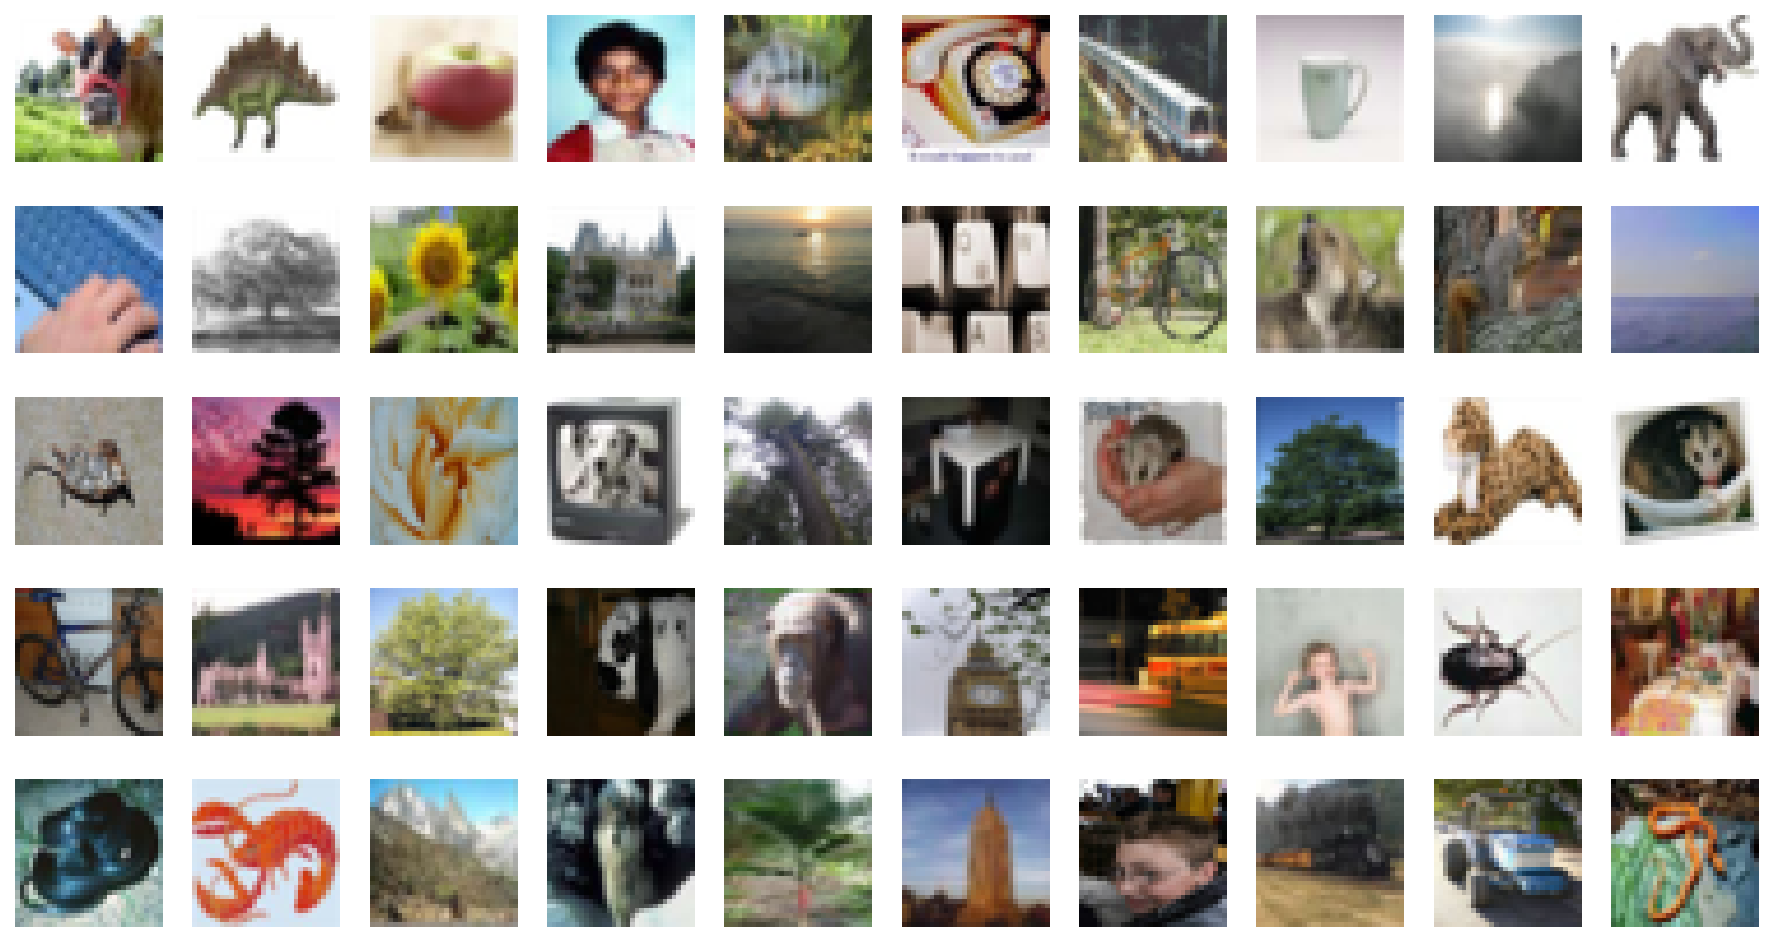
\includegraphics[width=\textwidth]{cifar100_samples.png}
    \caption{CIFAR-100 Sample Images \cite{37}}
    \label{fig:cifar100}
\end{figure}

The dataset is split into five successive tasks using the Split CIFAR-100 approach\cite{18}\cite{20} to simulate the CL scenario. The dataset has 20 mutually exclusive classes and therefore can be divided into tasks while preserving the original 5:1 train to test split ratio by using 10,000 training and 2,000 test images per task.

The system employs a TIL approach\cite{18} in which task identity is provided during both the inference and training processes. At the beginning of the training period for each task, a dedicated linear classifier with 20 output units is created. The ground truth task label constrains the categorization to the appropriate 20-class space by directing the input to the appropriate head. This approach avoids the issue of task identity inference while keeping the focus of representational forgetting in the shared backbone and adapter modules.

There is no access to previous task data, and tasks are given strictly sequentially. Following each task, the model is assessed on all tasks completed thus far, allowing for the calculation of the forgetting and BWT measures described in Section \ref{sec:4.5}.

All images are resized to 224 × 224 pixels using bilinear interpolation to meet the input requirements of the pre-trained ViT-Tiny backbone, which was trained at this resolution. The same preprocessing pipeline is applied to both training and test sets. Also, all images are normalized using ImageNet channel-wise mean (0.485, 0.456, 0.406) and standard deviation (0.229, 0.224, 0.225), consistent with the pre-training distribution of the ViT-Tiny backbone. Since ViT-Tiny was pre-trained on ImageNet at that resolution and its patch embedding layer anticipates a fixed $224\times224$ input, images for ViT-based models are resized from $32\times32$ to $224\times224$ pixels. Bilinear interpolation at this scale introduces a resolution mismatch between the pre-training distribution (natural 224×224 images) and the evaluation distribution (CIFAR-100 images upsampled from 32×32 to 224×224). While this upsampling may introduce interpolation artifacts and partially misalign with the spatial structure assumed by the positional embeddings learned during pre-training, this approach is standard practice in the CL literature when evaluating ViTs on CIFAR-scale benchmarks \cite{5}\cite{41}. The pre-trained positional embeddings are retained without modification, and the model adapts to the upsampled input through the adapter modules.

\begin{table}[h]
\centering
\caption{Split CIFAR-100 task configuration.}
\label{tab:4.1}
\small
\renewcommand{\arraystretch}{1.2}
\begin{tabular*}{\textwidth}{@{\extracolsep{\fill}}lccccc@{}}
\toprule
\textbf{Task} & \textbf{Class IDs} & \textbf{\# Classes} & \textbf{Train images} & \textbf{Test images} & \textbf{Setting} \\
\midrule
Task 1 & 0--19  & 20  & 10,000 & 2,000  & TIL \\
Task 2 & 20--39 & 20  & 10,000 & 2,000  & TIL \\
Task 3 & 40--59 & 20  & 10,000 & 2,000  & TIL \\
Task 4 & 60--79 & 20  & 10,000 & 2,000  & TIL \\
Task 5 & 80--99 & 20  & 10,000 & 2,000  & TIL \\
\midrule
Total  & 0--99  & 100 & 50,000 & 10,000 & Split CIFAR-100 \\
\bottomrule
\end{tabular*}
\end{table}

\section{Model Architecture Implementation}
\label{sec:4.3}
The architecture of every model configuration assessed in the ablation chain is described in depth in this section. Starting with the two simple fine-tuning baselines and moving on to the adapter-based architecture and its EWC-augmented variant, the three configurations are shown in increasing order of complexity. Every configuration builds upon the one before it, making it easy to see how each new element contributed to the outcome. 

\begin{table}[h]
\centering
\caption{Comparison of the evaluated model configurations.}
\label{tab:4.2}
\small
\setlength{\tabcolsep}{9pt}
\renewcommand{\arraystretch}{1.5}
\begin{tabular}{lcccc}
\toprule
\textbf{Configuration} & \textbf{Backbone} & \textbf{Adapter} & \textbf{EWC} & \textbf{Trainable Params} \\
\midrule
ResNet-18        & Unfrozen & No  & No  & 11.2M (100\%) \\
ViT-Tiny         & Unfrozen & No  & No  & 5.85M (100\%) \\
ViT+Adapters     & Frozen   & Yes & No  & 322K (5.5\%) \\
ViT+Adapters+EWC & Frozen   & Yes & Yes & 322K (5.5\%) \\
\bottomrule
\end{tabular}
\end{table}


\subsection{Baseline Models (ResNet-18 and ViT-Tiny)}
To determine reference points for catastrophic forgetting under naive sequential fine-tuning in which all parameters are updated on each task without using any forgetting mitigation strategy, two baseline models are assessed.

The first baseline is ResNet-18, a CNN with 11.2 million trainable parameters that consists of four residual stages with shortcut connections. ImageNet pre-trained weights are used to initialise ResNet-18, which is then successively fine-tuned on each task. Even while it performs well on basic image classification, the lack of a CL mechanism causes prior task knowledge to be quickly replaced when new tasks are added.

The second baseline is ViT-Tiny, which is a lightweight ViT that has 12 transformer blocks, 192 embedding dimensions, and three attention heads per block. It has 5.85 million parameters and is initialised with pre-trained ImageNet weights and then fine-tuned end-to-end like ResNet-18. Although ViT-Tiny has fewer parameters compared to ResNet-18, its use of a self-attention mechanism provides better and more transferable representations that result in significantly less forgetting without any explicit forgetting mitigation strategies, as shown in the experiment results in \hyperref[chap:5]{Chapter~\ref*{chap:5}}.

For both baselines, a separate linear classification head with 20 output units is initialized for each task and attached to the final layer output. To ensure a fair comparison, both ResNet-18 and ViT-Tiny are initialised with ImageNet-1k pre-trained weights. This controls for the effect of transfer learning, isolating the architectural and CL-methodological differences as the primary experimental variables. 
The same task incremental setup is used for both baselines, as described in Section \ref{sec:4.2}.

\subsection{ViT with Adapter Modules}
Adapter modules are used in the ViT-Tiny backbone network to implement a parameter-efficient form of CL to avoid the problem of catastrophic forgetting in the naive fine-tuning baselines. The idea is to completely freeze the pre-trained backbone network and task-specific learning is performed through tiny bottleneck modules inserted at each transformer block. This allows the network to adapt to new tasks using the minimum number of parameters while maintaining the generalised features learned during pre-training on the ImageNet dataset\cite{40}.

Each adapter follows a bottleneck design consisting of four operations applied in sequence: a LayerNorm normalises the input, a down-projection linear layer reduces the representation from the transformer's embedding dimension of 192 down to a bottleneck dimension of 64, a GELU activation introduces non-linearity, and an up-projection linear layer restores the original dimensionality of 192.  In order to reduce the initial effect of this module on the overall output of the frozen backbone, a residual connection is added around the adapter. Across all 12 blocks of ViT-Tiny, adapters are inserted after each full transformer block, after the feed-forward and self-attention sublayers. 

\begin{figure}[!htbp]
    \centering
    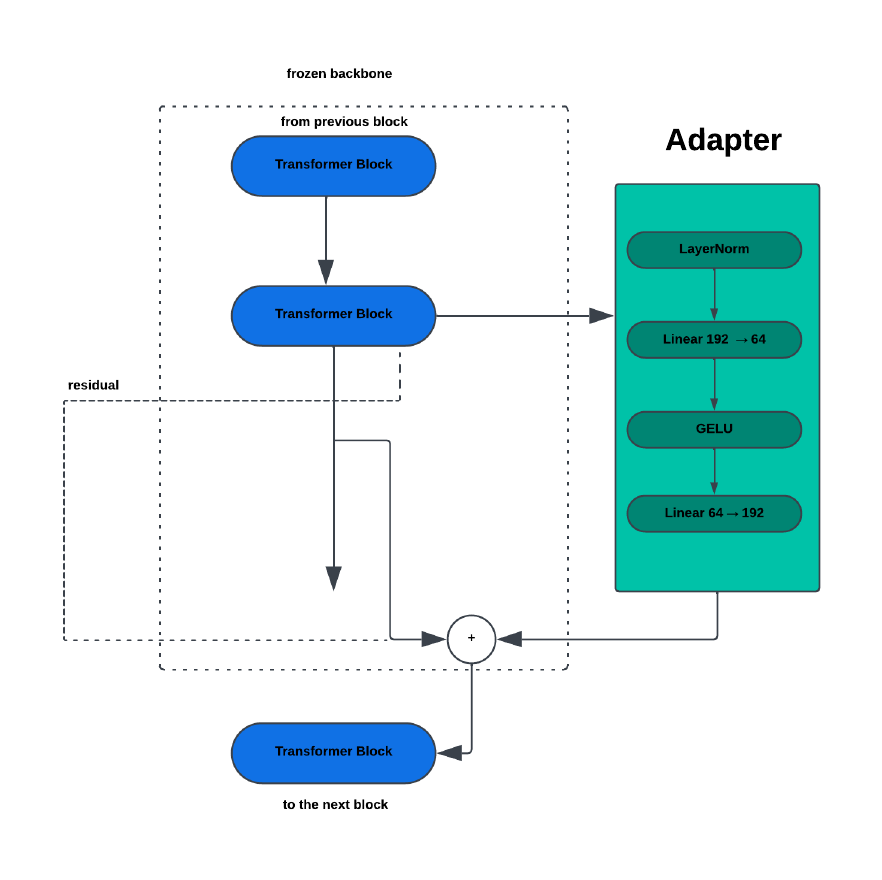
\includegraphics[width=\textwidth]{adapterPosition.png}
    \caption{Adapter Insertion Position}
    \label{fig:adapterPosition}
\end{figure}

Only the adapter parameters and the task-specific classification heads are updated during training, as the rest of the network is frozen. This leads to only around 321,000 parameters being left to update, which is around 5.5\% of all the parameters used by the ViT-Tiny network. The adapter configuration achieves significantly reduced forgetting compared to the fine-tuning baselines due to this extreme reduction in parameters.

\subsection{ViT with Adapters and EWC}
\label{sec:4.3.3}
In addition, EWC (EWC) is incorporated, which is a regularization method that better preserves parameters within adapters that were important for tasks previously learned. The adapter settings themselves are still vulnerable to overwriting when additional tasks are added, even when freezing the backbone already removes most forgetting. In order to overcome this, EWC penalises major deviations from parameter values that were considered significant during previous training phases.

Following training on each task, 500 randomly selected training examples are used to approximate the Fisher information matrix. A per-parameter importance estimate that shows how sensitive the task loss is to tiny changes in each adapter weight is obtained by accumulating squared gradients of the cross-entropy loss over batches and normalising them by the number of batches. Importantly, each task results in the creation of a distinct EWC object that stores the Fisher estimates for that task along with the parameter values at the end of training as anchors. The constraints from each previous task are given equal weight during subsequent training by adding the penalties from all previous EWC objects.
At each step, the total training loss is given by,

\begin{equation}
    \mathcal{L} = \mathcal{L}_{CE} + \frac{\lambda}{2} \sum_{k=1}^{t-1} \sum_{i} F_i^{(k)} {\left(\theta_i - \theta_i^{*(k)}\right)}^2
\end{equation}

where the regularization strength $\lambda$  is fixed at 1000 as stated before, $\mathcal{F}_i^{(k)}$ is the Fisher significance of the $i$-th parameter from task $k$, and $\theta_i^{*(k)}$ is the anchoring value of the $i$-th parameter after task $k$.

It is important to note that the classification heads are task-specific, and the backbone is frozen, so EWC regularization is only applied to the adapter parameters.

Also, the diagonal Fisher Information approximation used in this work stores one importance scalar per adapter parameter per completed task. With 322K adapter parameters and 5 tasks, the total Fisher storage overhead is approximately 6.3 MB (322K parameters × 4 bytes × 5 tasks), which is manageable relative to the model size ($\approx$23.4 MB for ViT-Tiny) and far less than the memory required for experience replay methods. The parameter-efficiency claim refers to the reduction in trainable parameters during gradient computation, which is a separate and compatible dimension from the Fisher storage overhead.

\section{Training Configuration}
\label{sec:4.4}
In this section, the training configuration that is common to all the configurations is presented, and the areas where the configurations differ are highlighted. In this part, the optimiser, the learning rate, the loss function, and the training process are presented sequentially. In addition, the reasons for the decisions made in the various configurations are presented. For instance, the EWC penalty in the adapter training and the reduced learning rate in the ViT-Tiny model.

\begin{table}[h]
\centering
\caption{Training settings used for each model configuration.}
\label{tab:4.3}
\small
\setlength{\tabcolsep}{4pt}
\renewcommand{\arraystretch}{1.2}
\begin{tabular*}{\textwidth}{@{\extracolsep{\fill}}lcccc@{}}
\toprule
\textbf{Parameter} & \textbf{ResNet-18} & \textbf{ViT-Tiny} & \textbf{ViT+Adapters} & \textbf{ViT+Adapters+EWC} \\
\midrule
Optimizer       & Adam  & Adam  & Adam  & Adam  \\
Learning Rate   & $1\times10^{-3}$  & $3\times10^{-5}$  & $1\times10^{-3}$  & $1\times10^{-3}$  \\
Batch Size      & 64    & 64    & 64    & 64    \\
Epochs per Task & 10    & 10    & 10    & 10    \\
$\lambda$ (EWC)   & ---   & ---   & ---   & 1000  \\
Fisher Samples  & ---   & ---   & ---   & 500   \\
\bottomrule
\end{tabular*}
\end{table}

\subsection{Optimizer and Learning Rate}
Adam optimizer\cite{38} with standard hyperparameters $(\beta_1 = 0.9, \ \beta_2 = 0.999, \ \varepsilon = 1 \times 10^{-8})$ and no learning rate scheduling is used to train all models. ViT-Tiny uses a much smaller learning rate of $3\times10^{-5}$ than ResNet-18, ViT + Adapters, and ViT + Adapters + EWC (which uses $1\times10^{-3}$). This is because fully unfrozen pre-trained transformers are known to be sensitive to large gradient updates and aggressive learning rates tend to distort the rich representations built during pre-training, so a more conservative value is used to preserve them while still allowing the model to adapt to each new task. Since the frozen backbone doesn't require gradient updates and eliminating it minimises needless computation, just the adapter parameters and task-specific classification heads are sent to the optimiser for adapter-based configurations.

\subsection{Loss Function}
The main training goal for all four configurations is cross-entropy loss, which is applied over the whole 100-class output layer. In line with the TIL setting outlined in Section \ref{sec:4.2}, task-specific logit masking limits predictions during evaluation to the 20 classes relevant to the present task. The combined objective described in Section \ref{sec:4.3.3} is obtained for the ViT + Adapters + EWC configuration by explicitly adding the EWC penalty term to the cross-entropy loss at each training phase. During training, neither loss scaling nor gradient clipping are used and instead, the regularization coefficient $\lambda$ controls the weighting between the task loss and the EWC penalty.

\subsection{Training Procedure}
Each task is trained for a total of ten epochs with a batch size of 64. There is no access to the data of the preceding tasks at any point during the training, and the tasks are always presented in the order specified. The accuracy matrix used in the computation of the metrics in Section \ref{sec:4.5} is obtained by evaluating the model on the test set of the completed tasks so far. In the case of the EWC variant, after training completes for each task but before training begins on the next task, the Fisher Information Matrix is computed using 500 randomly sampled examples from the just-completed task's training set. This ensures importance estimates reflect the converged model state. Unlike the case of the checkpoint, this ensures that the anchors and the importance values correctly capture the state of the model after it has converged.

\section{Evaluation Metrics}
\label{sec:4.5}
In this section, the three quantitative measures of the performance of the CL model are presented. These three measures provide an in-depth understanding of the extent of the ability of the various model configurations in retaining the previously learned information while still being able to learn new information. Each of the three measures represents a different dimension of the balance between stability and plasticity. 
\subsection{Average Accuracy}
The average accuracy is the main statistic that is used to measure the performance of the model. After completion of the entire task sequence by the model for training on the final task, it is defined as:

\begin{equation}
    \text{ACC} = \frac{1}{T} \sum_{i=1}^{T} A_{T,i}
\end{equation}
 
where $A_{T,i}$ is the accuracy for task $i$ after training on task $T$. This is a crucial statistic that can be used to measure the performance of CL over the entire task sequence because a model that has catastrophic forgetting performance on previous tasks will have low accuracy over the entire task sequence even if it has high accuracy on the latest task.

\subsection{Average Forgetting}
Average forgetting is a measure of the extent of the degradation of the performance of the previous task following training. For each task, the forgetting is calculated as the difference between the accuracy retained following the training of all the following tasks and the peak accuracy obtained on the task over the entire training process:

\begin{equation}
    \mathcal{F} = \frac{1}{T-1} \sum_{i=1}^{T-1} \left( \max_{t \leq T} A_{t,i} - A_{T,i} \right)
\end{equation}
 
Except for the last task, where there is no further training to induce any forgetting, the average is calculated over all the tasks. A value of zero indicates perfect retention, and higher values indicate catastrophic levels of forgetting.

Moreover, the forgetting metric measures degradation from post-training peak accuracy, not from initialization. For pre-trained models, a non-trivial zero-shot accuracy exists at initialization. However, this is not used as the reference point. The relevant question for CL evaluation is how much knowledge acquired during task-specific training is lost and not how much zero-shot transfer ability changes, which is a separate and complementary measure.

\subsection{Backward Transfer}
The impact of learning new tasks on the performance of previously learned ones is measured by BWT. It is described as the average difference between the accuracy reported just after the task was initially trained and the final accuracy on each previous task:

\begin{equation}
    \text{BWT} = \frac{1}{T-1} \sum_{i=1}^{T-1} \left( A_{T,i} - A_{i,i} \right)
\end{equation}
 
The hallmark of catastrophic forgetting is a negative BWT, which verifies that later training has deteriorated earlier task performance. To give a full view of how each configuration manages the stability-plasticity trade-off across the task sequence, BWT is reported in conjunction with average forgetting.

\section{Experimental Environment}
\label{sec:4.6}
For each experiment, Google Colaboratory is used, where a cloud-based NVIDIA GPU, usually T4, is available. The pre-trained ViT-Tiny model is loaded and instantiated via the library \enquote{timm}\cite{31}. PyTorch is used as a DL framework\cite{39}. At the beginning of each experiment, deterministic CUDA operations are enabled, and all random seeds in Python, NumPy, and PyTorch are set to 42. To ensure that the results are not affected by the task partition utilized during the main experiments, the cross-validation experiments presented in Section \ref{sec:5.4} are executed with three different seeds and different class orderings.
All models are implemented in Python and trained on the CIFAR-100 dataset, which can be retrieved through the Torchvision Datasets API. The EWC approach, the adapter modules, the evaluation procedure, and the metric computation are completely implemented from scratch without relying on any available CL library, which guarantees full transparency in the process.

\section{Conclusions}
\label{sec:4.7}
The entire experimental setup supporting the findings in \hyperref[chap:5]{Chapter~\ref*{chap:5}} has been covered in this chapter. In a TIL environment, the dataset and task setup adhere to the conventional split CIFAR-100 technique. From simple sequential fine-tuning baselines to a parameter-efficient adapter-based architecture enhanced with EWC regularization, four model configurations are assessed in an ablation chain. In order to isolate architectural and regularization decisions as the main variables, training is kept consistent across configurations whenever feasible using a shared batch size, number of epochs, and loss function. Together, the evaluation metrics, average accuracy, average forgetting, and BWT offer a thorough picture of each model's capacity to strike a balance between stability and flexibility over the five-task sequence.

\chapter{Testing and Evaluation}
\label{chap:5}
This chapter presents the results of the four model configurations evaluated on Split CIFAR-100 under the TIL framework described in \hyperref[chap:4]{Chapter~\ref*{chap:4}}. The experiments are structured as an ablation chain, allowing the contribution of each component — the pre-trained backbone, adapter modules, and EWC regularization to be assessed independently. Section \ref{sec:5.1} evaluates the two naive fine-tuning baselines, establishing the severity of catastrophic forgetting without any mitigation strategy. Section \ref{sec:5.2}  analyses the adapter-based configuration, examining how parameter-efficient fine-tuning affects forgetting and retention. Section \ref{sec:5.3} presents the results of full ViT + Adapters + EWC model, including a per-task breakdown and an ablation study isolating the contribution of EWC. Cross-validation results for three seeds are reported in Section \ref{sec:5.4} , and the results are discussed in Section \ref{sec:5.5} along with the reasons and limitations of the method being used. Section \ref{sec:5.6} concludes the chapter.

\section{Baseline Performance}
\label{sec:5.1}
The two baseline models, ResNet-18 and ViT-Tiny are assessed using naive sequential fine-tuning, in which no forgetting mitigation mechanism is used and all parameters are updated on each task. The severity of catastrophic forgetting in the absence of any CL mechanism is established by these results, which also serve as benchmarks for comparing adapter-based systems.

With an average forgetting rate of 69.17\% and a BWT rate of negative 69.17\%, the average accuracy achieved by the ResNet-18 model is 24.22\%.This further proves the point that the addition of new tasks causes the knowledge learned from the previous task to almost completely collapse, as the model retains very little knowledge towards the end, even if it is doing reasonably well on each task after being trained on them.

On the other hand, the ViT-Tiny model achieves an average accuracy of 41.91\%, an average forgetting rate of 63.26\%, and a BWT rate of negative 63.26\% despite being fine-tuned in the same naive way. The richer representations transferred through the self-attention mechanism are the main contributing factor to the improved performance over the ResNet-18 model. Even in the absence of a mitigation strategy, the global context captured by the transformer blocks appears to generalize better than the local features captured by convolutional operations in ResNet-18, resulting in less forgetting.

In sequential task settings, the baseline experiments exhibit significant catastrophic forgetting, which further supports the requirement for task-specific CL mechanisms. 
\section{ViTs with Adapters}
\label{sec:5.2}
The adapter-based setup significantly outperforms both baselines with an average accuracy of 76.93\%, an average forgetting of 19.91\%, and a BWT rate of negative 19.91\%. This finding shows that a very successful method for reducing catastrophic forgetting in a CL environment is to freeze the pre-trained backbone and route task-specific learning through lightweight bottleneck adapters.

Architectural factors are the main cause of this improvement. The rich representations acquired during ImageNet pre-training are maintained throughout the task sequence by keeping the backbone frozen. The adapter parameters are the sole location in which new task knowledge is represented, and they are sparse, such that they do not significantly influence previously learned representations from previous tasks. The significant decrease in forgetting when compared to the naive fine-tuning baselines is caused by this structural division between task-specific trainable modules and shared frozen features.

But it's important to take into account that some forgetting still happens. Since the same set of adapters is updated for each of the five tasks, the adapter parameters themselves are vulnerable to overwriting, with an average forgetting of 19.91\%. It is also possible for later task-specific adaptation to override previous ones, and this is because there is no mechanism in place that stops adapter weights from changing. To further stabilize knowledge retention, EWC regularization, which directly affects adapter parameters, is added in the final configuration due to residual forgetting.
\section{ViTs with Adapters and EWC}
\label{sec:5.3}
This section presents the results of the final and most complete configuration, which combines the frozen ViT-Tiny backbone, bottleneck adapter modules, and EWC regularization applied exclusively to the adapter parameters. This configuration represents the primary contribution of the thesis, and its results are analysed in terms of overall performance, per-task behaviour, and the isolated contribution of EWC.

\subsection{Overall Performance}
Amongst all four configurations, the ViT + Adapters + EWC configuration has yielded the best results, with an average accuracy of 90.59\%, an average forgetting of 2.01\%, and a BWT rate of negative 1.85\%. When EWC regularization is added to the adapter-based model, forgetting is significantly reduced (from 19.91\% to 2.01\%) and average accuracy is increased by about 14 percentage points. This finding demonstrates that EWC and adapter freezing are complementing mechanisms, EWC prevents the adapter parameters from being overwritten when new tasks are added, while the frozen backbone removes forgetting in the shared representations.

The near-zero BWT rate of negative 1.85\% suggests that learning subsequent tasks has essentially no negative influence on earlier task performance. This level of stability is rare in CL environments without the use of experience replay or task-specific parameter isolation. This demonstrates that, since regularization occurs precisely where forgetting would have occurred, using EWC on merely the adapter parameters, rather than the whole network, is computationally efficient and highly effective.

The progressive improvement across configurations is attributable to the cumulative effect of each design decision rather than pre-training alone. The naive ResNet-18 baseline, which also uses ImageNet pre-training, achieves only 24.22\% accuracy demonstrating that pre-training quality alone does not determine CL performance. The subsequent improvements from ViT architecture, adapter modules, and EWC regularization each provide measurable, isolatable gains as evidenced by the ablation chain in Section \ref{sec:5.3.3} .

\begin{figure}[!htbp]
    \centering
    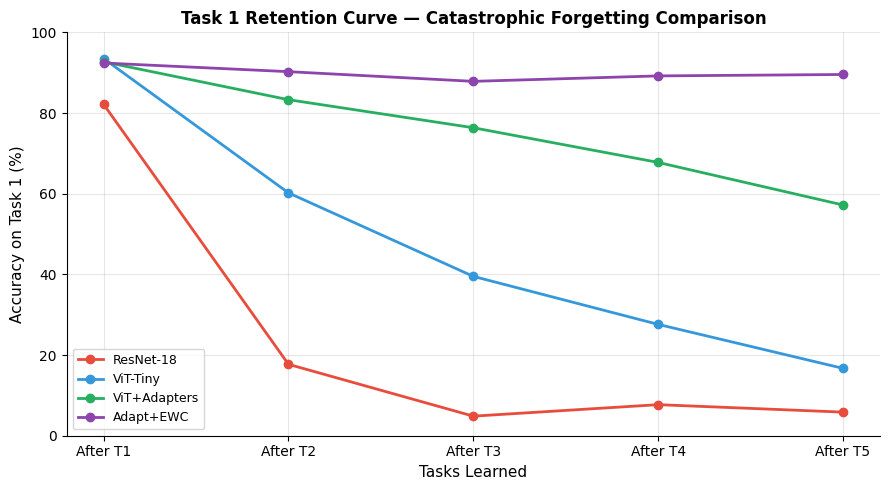
\includegraphics[width=\textwidth]{Task1RetentionCurveCatastrophicForgettingComparison.png}
    \caption{Task 1 Retention Curve Catastrophic Forgetting Comparison}
    \label{fig:forgetting_graph}
\end{figure}

\begin{figure}[!htbp]
    \centering
    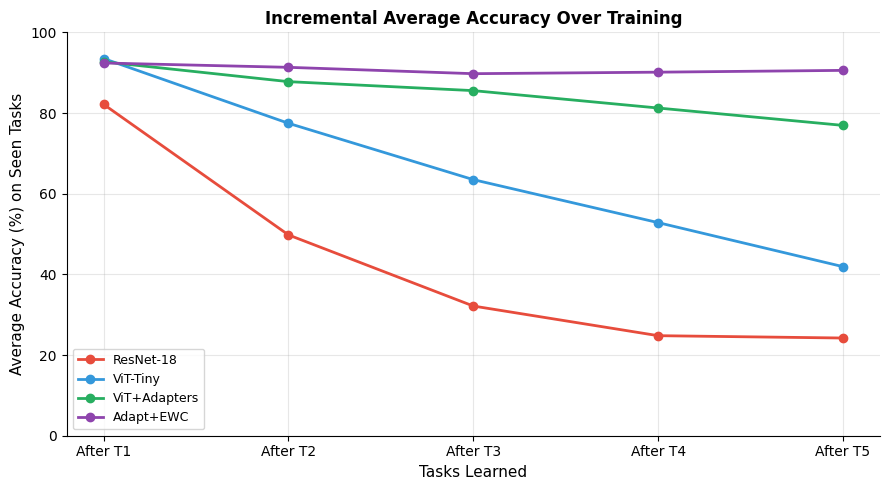
\includegraphics[width=\textwidth]{IncrementalAverageAccuracyOverTraining.png}
    \caption{Incremental Average Accuracy Over Training}
    \label{fig:IncrementalAverageAccuracyOverTraining}
\end{figure}

\subsection{Per-Task Breakdown}
The evolution of this process of forgetting can be observed if we examine the performance individually for each task. As the tasks are presented earlier, a slight increase is observed in the rate of forgetting compared to those presented later. The rate of forgetting for the ViT + Adapters + EWC configuration continues to be low for all tasks, and the values are similar for all tasks. Naturally, this is expected to be the case because it is likely for previous tasks to be influenced by subsequent training phases. Figure \ref{fig:accuracyheatmap_baseline} , Figure \ref{fig:accuracyheatmap_adapt} and Figure \ref{fig:accuracyheatmap_adapt_ewc} represent Accuracy heatmaps for all 4 models.


\begin{figure}[h]
    \centering
    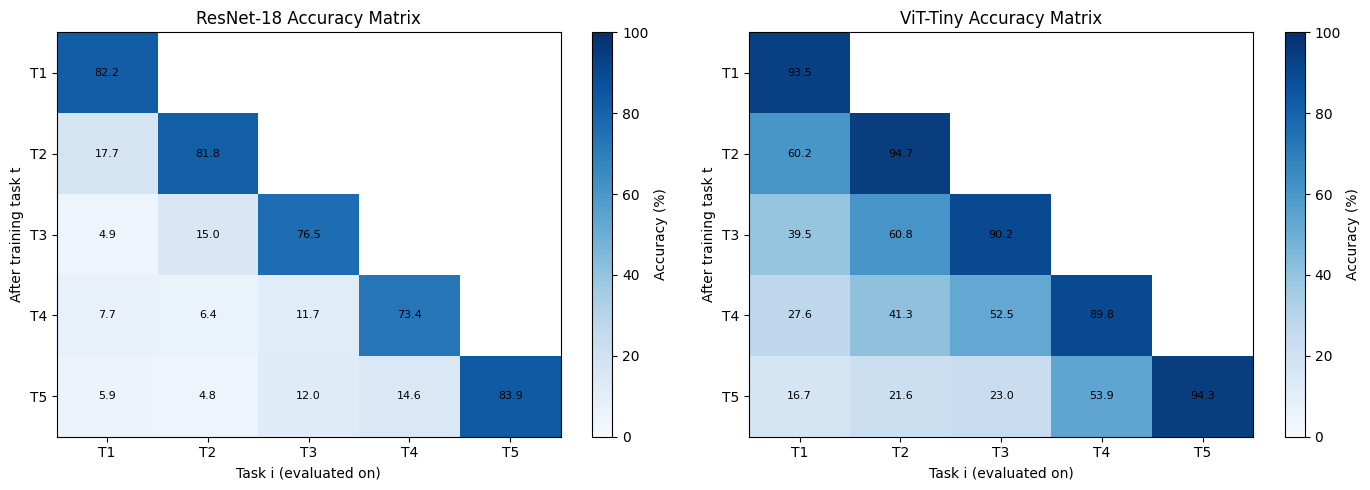
\includegraphics[width=\textwidth]{accuracyheatmap_baseline.png}
    \caption{Accuracy Heatmap for baseline models}
    \label{fig:accuracyheatmap_baseline}
\end{figure}

\begin{figure}[h]
    \centering
    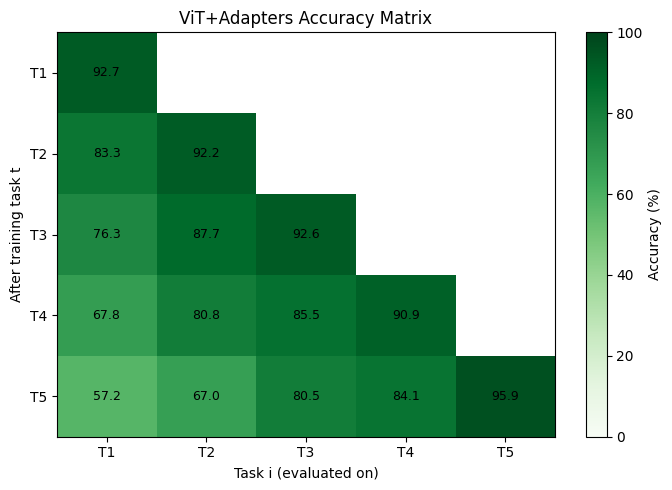
\includegraphics[width=\textwidth]{accuracyheatmap_adapt.png}
    \caption{Accuracy Heatmap for ViT + adapters}
    \label{fig:accuracyheatmap_adapt}
\end{figure}

\begin{figure}[h]
    \centering
    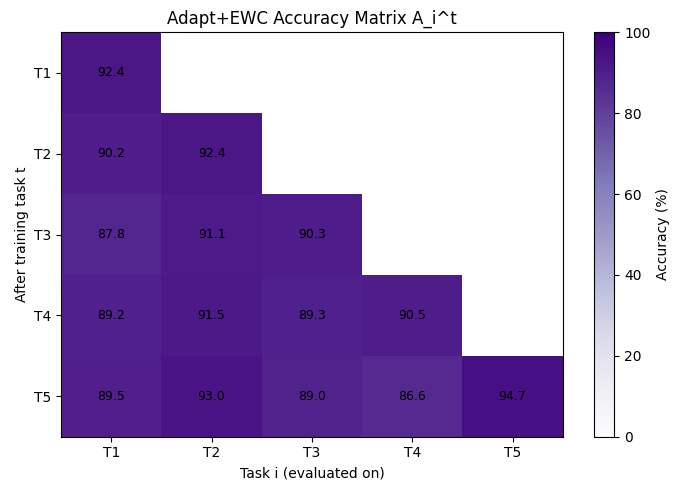
\includegraphics[width=\textwidth]{accuracyheatmap_adapt_ewc.png}
    \caption{Accuracy Heatmap for ViT + adapters + EWC}
    \label{fig:accuracyheatmap_adapt_ewc}
\end{figure}

For the baseline models and the adapter-only configuration, a clear gradient is observed in the rate of forgetting, with the highest degradation observed for Task 1 and the lowest for Task 4, consistent with the expectation that earlier tasks are more likely to be overwritten by subsequent training. However, this gradient collapses when EWC is incorporated. The per-task forgetting for the EWC configuration is [2.85\%, 0.00\%, 1.30\%, 3.90\%], which does not follow a monotonic pattern and Task 2 experiences zero forgetting while Task 4 shows the highest degradation of 3.90\%. This non-monotonic behaviour suggests that EWC's protection is driven by Fisher importance rather than task order, with some tasks' adapter weights being more susceptible to interference depending on the specific feature distributions encountered. Importantly, despite this variation, forgetting remains low and consistent across all tasks, with a maximum of only 3.90\%, confirming that EWC effectively controls catastrophic forgetting across the entire task sequence. This is consistent with the theory that, as tasks are presented earlier, the likelihood that this representation may be overwritten is increased. The gradient, however, collapses when we incorporate EWC, and forgetting remains low and consistent across tasks. While one might expect a bias in favor of more recently learned tasks, as would occur if importance estimates from earlier tasks were allowed to decay, we observe a uniform behavior, demonstrating that the EWC penalty effectively covers the entire task history.

\subsection{Ablation Study: Contribution of EWC}
\label{sec:5.3.3}
In this regard, the results obtained by the Adapter-only and the Adapter + EWC methods are directly compared to determine the effectiveness of the EWC method. 

\begin{figure}[!htbp]
    \centering
    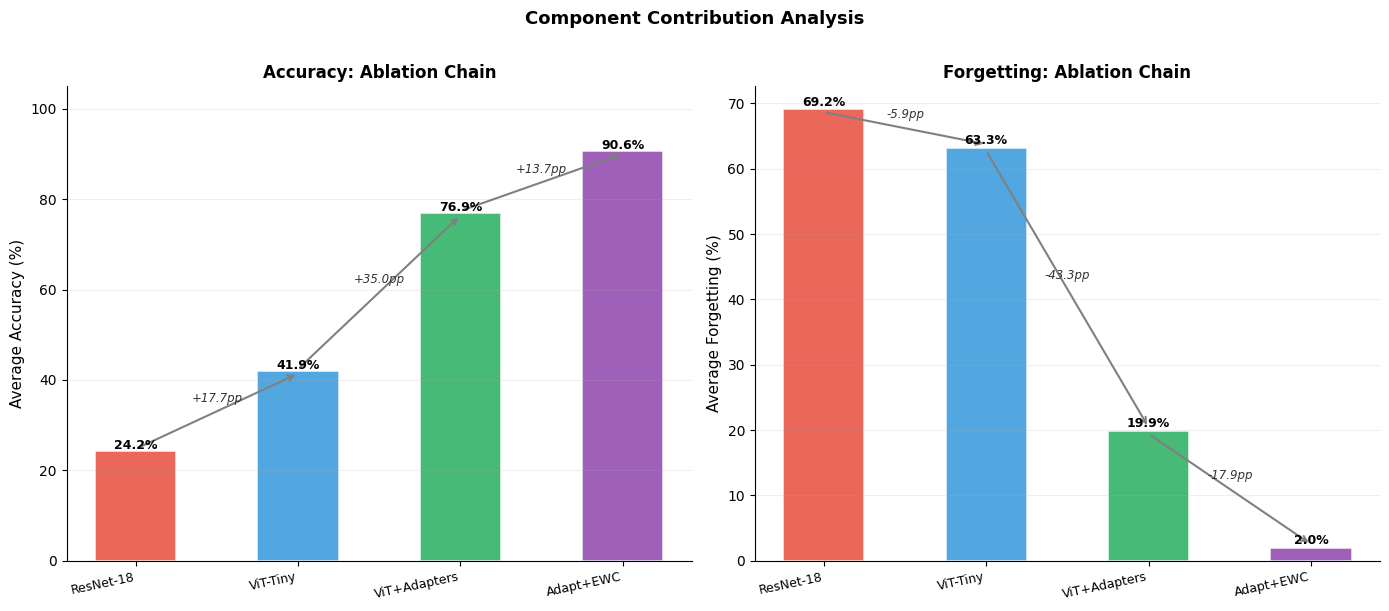
\includegraphics[width=\textwidth]{ComponentContributionAnalysis.png}
    \caption{Component Contribution Analysis}
    \label{fig:AblationStudy}
\end{figure}


It is observed that the use of the EWC method improves the accuracy by 13.66 percentage points, i.e., from 76.93\% to 90.59\%, while reducing the average forgetting by 17.9 percentage points, i.e., from 19.91\% to 2.01\%, without changing the backbone model, adapter model, training time, and batch size. The improvement from the Adapter-only to the Adapter+EWC configuration is substantially larger than the cross-validation standard deviation of ±1.78\%, suggesting the improvement is robust and not attributable to random variance. Formal statistical significance testing (e.g., paired t-test) across a larger number of seeds would provide additional rigor and is recommended for future work.

Crucially, plasticity is not sacrificed in order to get the improvement. The high average accuracy shows that the model is still learning each new task efficiently. This indicates that, when applied solely to the 322K adapter parameters, the regularization strength of $\lambda$=1000 effectively balances stability and plasticity, limiting the adapter weights sufficiently to prevent forgetting without limiting their ability to encode new task knowledge. The outcome supports the design decision to apply EWC solely to the adapter settings rather than the entire network.

\begin{table}[h]
\centering
\caption{Main results summary.}
\label{tab:main_results_summary}
\small
\renewcommand{\arraystretch}{1.2}
\begin{tabular*}{\textwidth}{@{\extracolsep{\fill}}lccc@{}}
\toprule
\textbf{Model} & \textbf{Avg Accuracy} & \textbf{Avg Forgetting} & \textbf{BWT} \\
\midrule
ResNet-18           & 24.22\% & 69.17\% & -69.17\% \\
ViT-Tiny            & 41.91\% & 63.26\% & -63.26\% \\
ViT + Adapters        & 76.93\% & 19.91\% & -19.91\% \\
ViT + Adapters + EWC    & 90.59\% & 2.01\%  & -1.85\% \\
\bottomrule
\end{tabular*}
\end{table}


\section{Cross-Validation Results}
\label{sec:5.4}
The ViT + Adapters + EWC configuration is assessed using a three-seed cross-validation methodology to ensure that the results presented in Section \ref{sec:5.3} are not an artefact of a specific class ordering or random initialization. Performance is tested and averaged over three different task partitions created by each seed's unique random class-to-task assignment.

\begin{figure}[!htbp]
    \centering
    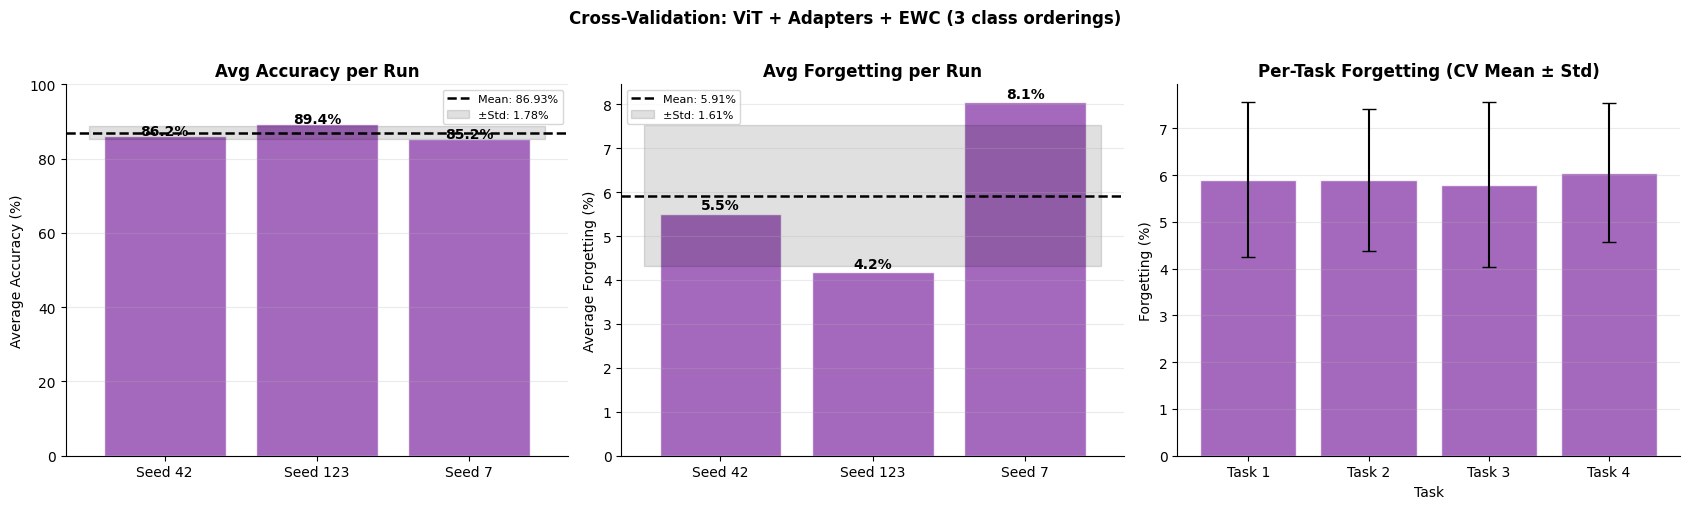
\includegraphics[width=\textwidth]{CrossValidation.png}
    \caption{Cross-Validation: ViT + Adapters + EWC (3 class orderings)}
    \label{fig:Cross-Validation}
\end{figure}

The model obtains an average accuracy of 86.93\% with a standard deviation of ±1.78\% and an average forgetting of 5.91\% with a standard deviation of ±1.61\% for all three seeds. This is in agreement with the accuracy rate of 90.59\%, and forgetting of 2.01\% using seed 42 in the primary test. The findings are not affected by the classes being grouped together within a task, and the low standard deviations indicate consistency in different task orders.

Since different class orderings bring varying degrees of inter-task similarity that can affect how readily the model transitions between tasks, it is expected that the cross-validation would show slightly lower mean accuracy and higher mean forgetting than the initial run. However, the cross-validation findings verify that the ViT + Adapters + EWC configuration generalizes robustly across task configurations and that the excellent performance reported in the primary experiment is not due to a favorable random seed, but rather to the overall effectiveness of the approach. 

Formal statistical significance testing was not conducted due to the limited number of seeds. However, the improvement from Adapter-only to Adapter+EWC (13.66 percentage points in accuracy, 17.9 percentage points in forgetting) substantially exceeds the measured cross-validation standard deviation (±1.78\% accuracy, ±1.61\% forgetting), suggesting the difference is robust to random variation in task ordering and class partitioning. Rigorous significance testing across a larger number of seeds is recommended for future work.

\begin{table}[h]
\centering
\caption{Results across three experimental runs with different random seeds.}
\label{tab:multi_run_results}
\small
\renewcommand{\arraystretch}{1.2}
\begin{tabular*}{\textwidth}{@{\extracolsep{\fill}}lcccc@{}}
\toprule
\textbf{Run} & \textbf{Seed} & \textbf{Avg Accuracy (\%)} & \textbf{Avg Forgetting (\%)} & \textbf{BWT (\%)} \\
\midrule
1        & 42  & 86.19 & 5.51 & -5.51 \\
2        & 123 & 89.39 & 4.18 & -4.18 \\
3        & 7   & 85.22 & 8.05 & -8.05 \\
\midrule
\textbf{Mean} & --- & \textbf{86.93} & \textbf{5.91} & \textbf{-5.91} \\
\textbf{Std}  & --- & \textbf{1.78}  & \textbf{1.61} & \textbf{1.61} \\
\bottomrule
\end{tabular*}
\end{table}

\section{Discussion}
\label{sec:5.5}
The results from all the configurations show an improvement in the accuracy and knowledge retention, and this improvement is consistent and progressive as each part is added. The section discusses the underlying reasons behind the success achieved by the last configuration and the limits of the method, assumptions, and constraints, among them, that might affect the generalization of the results outside the experimental setting.

\begin{figure}[!htbp]
    \centering
    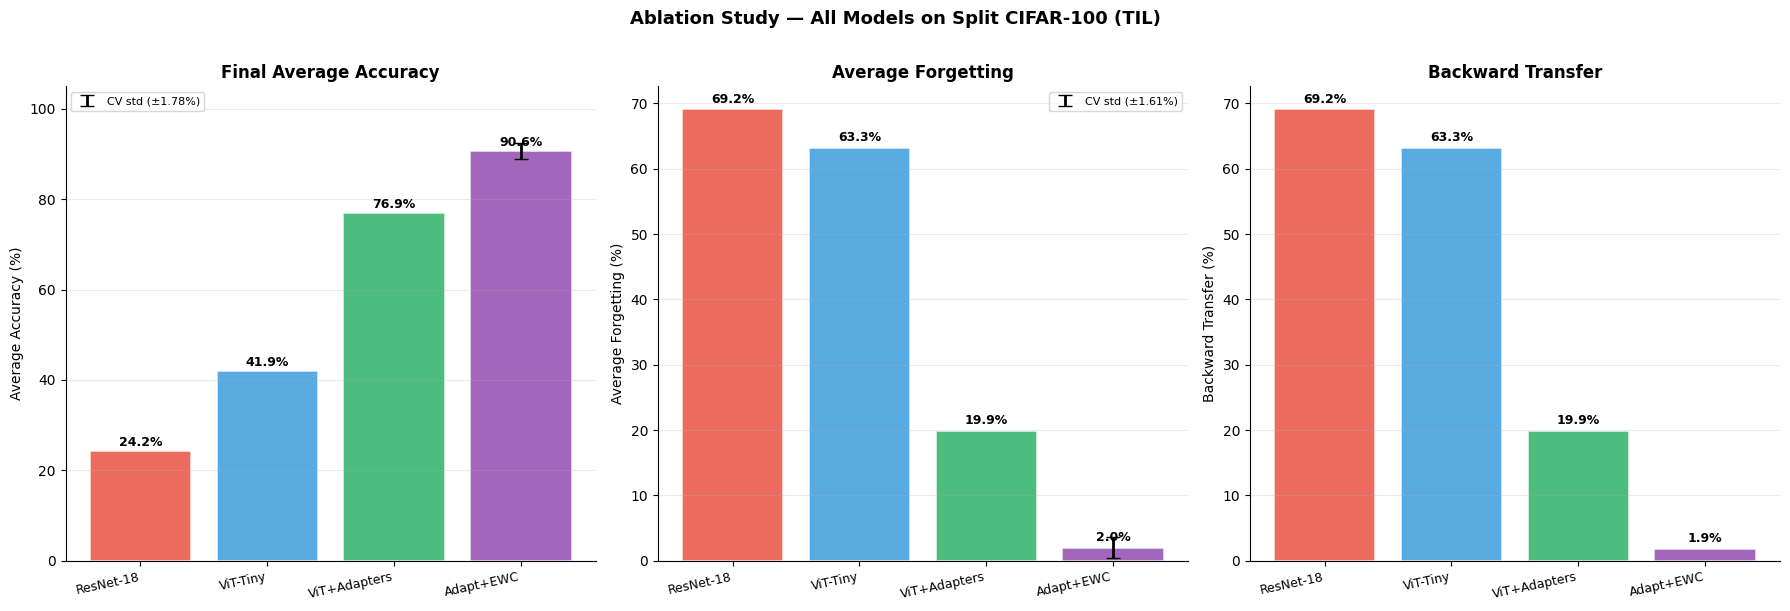
\includegraphics[width=\textwidth]{MetricsResults.png}
    \caption{All Models on Split CIFAR-100 (TIL)}
    \label{fig:MetricsResults}
\end{figure}

\subsection{Why the Method Works}
The complementing interaction between three design decisions, ImageNet pre-training, adapter-based parameter efficiency, and EWC regularization, is responsible for the ViT + Adapters + EWC configuration's outstanding performance.

Pre-training forms the foundation of the approach. The ViT-Tiny model is provided with rich and generally applicable visual representations, which are appropriate for the diverse class distributions encountered in the Split CIFAR-100 data set. This is shown by the fact that, despite having fewer total parameters, the naive ViT-Tiny baseline outperforms the ResNet-18 model by approximately 18 percentage points on average accuracy. The most important factor in forgetting is eliminated without any additional computational cost by freezing the visual representations, thus ensuring their integrity along the entire task sequence.

While the TIL setting provides task identity at inference, it does not eliminate the CL challenge studied in this thesis. The separate output heads prevent output-level confusion but do not protect the shared adapter parameters from sequential interference. The baseline forgetting rates of 63.26\% (ViT-Tiny) and 69.17\% (ResNet-18), both of which use separate heads demonstrate that representational forgetting in the shared parameter space remains a substantial challenge in TIL. The distinction from multi-task learning is also important: joint training on all tasks simultaneously is not performed at any point and tasks are presented strictly sequentially with no access to prior task data, which is what induces forgetting and necessitates the CL methods evaluated.

Next, the adapter modules provide an organized way to perform task-specific learning within the frozen visual representations. The risk of interference from new task training with previous adaptations is reduced significantly by limiting the gradients to 5.5\% of the total parameter count. Zero initialization of the up-projection weights ensures that the adapter is effectively an identity function, and the use of a bottleneck structure ensures that the adapter learns its deviation from the identity function.

The residual forgetting that occurs within the adapter parameters is handled by EWC. EWC effectively combines all the knowledge from the previous tasks into soft constraints, ensuring they are satisfied throughout the entire training process, by using the Fisher information matrix to assess the importance of the parameters and penalizing the deviation from the previously learned values. By using EWC only on the adapter parameters, as opposed to the entire model, the regularization is kept efficient and the parameters are the ones where the forgetting actually occurs.

A potential concern with applying EWC to adapter parameters is that, unlike backbone weights, adapter parameters are randomly initialized and carry no prior knowledge before Task 1 training. This raises the question of what EWC is protecting. The answer is that after Task 1 training, the adapter parameters encode Task 1-specific feature transformations. EWC then protects these learned transformations from being overwritten during Task 2 training, it is not protecting pre-existing knowledge, but rather task-acquired knowledge within the adapter. The Fisher Information computed after Task 1 reflects which adapter weights are most critical for Task 1 performance, and EWC constrains those weights during subsequent tasks. This is consistent with the original EWC formulation, which protects parameters important for a previously learned task regardless of how those parameters were initialized. Also, The adapter-only configuration achieves 19.91\% average forgetting, showing that freezing the backbone and restricting learning to shared adapter parameters is not sufficient to eliminate interference across tasks. Adding EWC reduces average forgetting to 2.01\%, corresponding to an approximately 90\% relative reduction. This result shows that adapters and EWC are complementary rather than redundant. Adapters reduce the scope of parameter updates, while EWC protects the most important adapter weights from being overwritten.

By tackling the problem of catastrophic forgetting from different levels in the neural network, these three components are combined to form a system that is flexible enough to learn new tasks and yet stable enough to retain the previously learned task information.

\subsection{Limitations and Future Work}
While the results are quite impressive, there are a few things to be aware of. First and foremost, the experiments are conducted in the TIL scenario, in which task identification is provided to the model during inference time. However, for the CIL scenario, in which the model has to learn the appropriate task head on its own without any identification, is used, then the performance of the model might decrease. This is the most favorable CL scenario. TIL is considered the most tractable CL setting because task identity is provided at inference time, enabling task-specific output head selection and reducing the difficulty of the forgetting problem compared to CIL. The combination of TIL with a frozen backbone and adapter modules means that parameter isolation operates at two levels simultaneously: the frozen backbone prevents backbone-level forgetting entirely, while the task-specific heads prevent output-level confusion. It could therefore be argued that the low forgetting observed is partly a structural property of the experimental design rather than solely a consequence of the proposed method. This is an acknowledged limitation, and future work should evaluate whether the same approach generalizes to CIL, where task identity is unavailable at inference time and the model must discriminate among all classes seen so far without any task oracle.

Second, all 12 transformer blocks in the adapter architecture have a fixed bottleneck dimension of 64. However, no hyperparameter tuning was done to try to improve this number, so it's possible that different tasks or blocks would benefit from different bottleneck sizes. Additionally, instead through hyperparameter tuning, the strength of EWC regularization was set at $\lambda$ = 1000, based on values often reported in literature, though further hyperparameter tuning could yield more improvements.

Third, a partial estimate of variance is given through the restriction of cross-validation to three seeds. A more statistically sound estimate of generalization across partitions would result from a greater number of seeds and task orderings.

Fourth, the resolution gap between CIFAR-100 (32×32) and the ViT-Tiny's pre-training resolution (224×224) represents a potential confound. Upsampling via bilinear interpolation may distort fine-grained visual features and reduce the effective utility of the pre-trained representations. Attention map analysis to verify that the model attends to meaningful image regions rather than upsampling artifacts was not conducted and remains an avenue for future work. However, the high average accuracy (90.59\%) and low forgetting (2.01\%) achieved despite the resolution gap suggest that the pre-trained representations remain functional after bilinear upsampling. The upsampling approach used here is consistent with standard practice in the CL literature \cite{5}\cite{41} for ViT evaluation on CIFAR-scale benchmarks.

Fifth, The experimental design does not include a ResNet-18 with adapter modules baseline. While adapter-based PEFT has been applied to CNN architectures such as ResNet in prior work \cite{15}\cite{rebuffi}, the architectural motivation is considerably stronger for Transformers. The modular block structure of ViTs, comprising stacked, identical layers each with well-defined attention and feed-forward sublayers provides natural, standardized insertion points for bottleneck adapter modules \cite{15} \cite{32}. CNNs lack this uniform block structure and convolutional stages vary in spatial resolution and channel dimensionality across the network, making principled adapter placement less straightforward and less studied in the CL context\cite{rebuffi}. Including ResNet + Adapters would clarify whether the performance gains observed are attributable to the adapter mechanism specifically or to the ViT architecture more broadly. This comparison is recommended for future work.

Sixth, the Split CIFAR-100 benchmark is a fairly well-controlled environment with five tasks, each with 20 classes. Real-world CL scenarios typically involve longer task sequences, greater distributional shift between tasks, and tasks that are not cleanly separable into equal-sized partitions.  Clearly, there remains much work to be done in exploring how generalizable this work is to realistic scenarios.

Finally, all state-of-the-art comparisons in this thesis are contextual rather than quantitative and direct comparison against methods such as L2P\cite{5}, DualPrompt\cite{41}, and SLCA\cite{slca} is not feasible due to fundamental differences in CL scenario, backbone size, and pre-training data, as discussed in Section \ref{sec:1.2}.
\section{Conclusions}
\label{sec:5.6}
In this chapter, the evaluation of four model configurations on the Split CIFAR-100 dataset using a CL approach was conducted. From the results obtained, a significant and consistent improvement in the model’s performance can be observed along the ablation chain with the inclusion of a certain component resulting in measurable values of forgetting and accuracy.

With the ResNet-18 and ViT-Tiny models achieving 24.22\% and 41.91\% accuracy on the Split CIFAR-100 dataset, the naive fine-tuning baselines highlighted the severity of catastrophic forgetting without the aid of a CL approach. With the inclusion of the adapter modules, the average accuracy improved to 76.93\%, and the average forgetting decreased from 63.26\% to 19.91\%, proving parameter-efficient fine-tuning with a frozen backbone of a pre-trained model to be a highly effective approach to the CL problem. With a final average accuracy of 90.59\%, the addition of EWC regularization further decreased forgetting to just 2.01\%. This result was confirmed by cross-validation over three seeds, which yielded a mean accuracy of 86.93\% ± 1.78\% and a mean forgetting of 5.91\% ± 1.61\%.

When combined, these findings imply that a frozen pre-trained backbone, lightweight adapter modules, and EWC regularization provide a practical and computationally efficient way to address catastrophic forgetting in ViT models. While stressing restrictions related to the task-incremental setting, fixed hyperparameters, and benchmark scope that should be taken into account when interpreting these results, the discussion in Section \ref{sec:5.5} identified the complimentary nature of these components as the primary driver of performance.

\chapter{Conclusions}
\label{chap:6}
This thesis work addressed catastrophic forgetting in pre-trained ViTs using a task-incremental CL framework, which is an underexplored field considering that the majority of CL research has traditionally concentrated on CNN-based architectures. The work showed that combining a frozen pre-trained ViT backbone with lightweight bottleneck adapter modules and EWC regularization provides a highly effective solution to catastrophic forgetting in vision tasks via a structured ablation chain on Split CIFAR-100. The frozen backbone maintains shared representations, the adapters offer task-specific learning capability, and EWC shields the adapter parameters from interference between tasks. Each component tackles forgetting at a complimentary level. Although the use of EWC and adapter modules has been studied individually in the existing literature, the novelty of this study lies in the application of these methods to ViTs in a CL scenario.  The findings demonstrate that substantial knowledge retention can be achieved without the computational burden of complete model fine-tuning or experience replay when parameter-efficient fine-tuning is combined with targeted regularization.The task-incremental setting, fixed hyperparameters, and benchmark scope are still limitations. Future research could expand the evaluation to class-incremental settings, larger ViT variations, and more intricate task sequences.

\backmatter
\phantomsection

\bibliographystyle{IEEEtran}
\bibliography{references}

\end{document}